\documentclass[a4paper,11pt]{article} % remove draft to include figures
\usepackage{amsmath}
\usepackage{graphicx,afterpage,float,subcaption,geometry,epsfig,tikz,pgfplots,bm,authblk}
\usepackage{fancyvrb,relsize,xcolor}
\usepackage[section]{placeins}
\usepackage{url}
\usetikzlibrary{positioning,shapes,shadows,arrows,fit,backgrounds}
\geometry{margin=2.5cm}

\usepackage[round]{natbib}
\usepackage[multiple]{footmisc}

\graphicspath{{img/}}

% 2.	Scope of Work: Develop simulations and software to plan sampling so it provides estimates with a desired coefficient of variation that is less than 30%
% Deliverable: Report detailing simulations and guiding software codes to run specific analyses pertaining to snow leopard population estimation

% \pgfplotstableread{xxx2.txt}{\datatable}
%
% Style to select only points from #1 to #2 (inclusive)
%\pgfplotsset{choose between/.style 2 args={
%    x filter/.code={
%        \ifnum\coordindex<#1\def\pgfmathresult{}\fi
%        \ifnum\coordindex>#2\def\pgfmathresult{}\fi
%    }
%}}
%
%\pgfplotsset{
%    cycle list={red\\yellow\\green\\},
%}

\setcounter{tocdepth}{2} % Show sections

\begin{document}
\baselineskip = 1.3\baselineskip 
\title{Snow leopard macro-level survey design and inference}
\author[1]{Ian Durbach\footnote{Corresponding author: \texttt{id52@st-andrews.ac.uk}}}
\author[1]{David Borchers}
\affil[1]{Centre for Research into Ecological and Environmental Modelling, University of St Andrews, UK}
\date{\today}
\maketitle

% Deliverable: Report detailing simulations and guiding software codes to run specific analyses pertaining to snow leopard population estimation

\tableofcontents

\section{Overview}
This report documents simulations and guiding software developed to assist the design of large-scale camera trap surveys such as those done as part of the Population Assessment of the World's Snow Leopards (PAWS). Large-scale camera trap surveys consist of two levels of design decision. At the higher or ``macro'' level, there is a decision about which parts of the entire snow leopard range to survey. Here the survey instrument can be thought of as an entire array of e.g.\ 30-60 cameras, or more specifically by the mesh defining the survey area around the camera trap array. What we want to determine is where, roughly, to place each of the camera arrays, without worrying at this stage about exactly where each camera will be placed. Once the broad survey areas have been defined, a second or ``micro'' level design is used within each of the survey areas to determine the location of each camera trap. The current report is focussed on the selection of survey regions i.e.\ on macro-level design issues.

A fundamental requirement of the PAWS approach is that study areas should be chosen according to the principles of statistical survey design. In practice this means being able to quantify the probability of including any potential survey site in the final sample. Without these probabilities it is impossible to objectively know how representative the surveyed areas are of the entire range, and thus impossible to extrapolate from the areas that are surveyed by camera traps to those areas that were not sampled. As only a small proportion of snow leopard range will be sampled by PAWS, it is crucial to be able to extrapolate beyond the surveyed regions. Currently, survey regions are often chosen on the basis of expert knowledge about where snow leopards are most likely to be found. This approach does not provide inclusion probabilities and the representativeness of the chosen areas is subjective and open to debate and disagreement; there is no objective way of going from estimates of snow leopard abundance within the regions covered by camera traps to range-wide estimates of snow leopards. For this reason \cite{McDonald2012} calls these designs ``non-scientific''.

In addition to this fundamental requirement, there are some additional practical requirements for any macro-level design. Firstly, as it is impossible to know in advance how many camera trap surveys will be done, we need an approach able to add survey areas later on in such as way that preserves the efficiency of the design. Secondly, the design must allow for stratification by country and be reproducible within any of the snow leopard range countries. Finally, the design should avoid areas that are inaccessible to humans or that are not viable snow leopard habitat i.e.\ are {\it known} not to be occupied by snow leopards (note that this is not the same as ``low probability'' or ``poor habitat'' areas, which {\it must}, according to statistical design principles, be available for potential selection).

The approach and accompanying software provided here has two main goals:
\begin{enumerate}
\item To provide an approach to allow researchers to calculate the expected efficiency of any candidate design selected according to statistical design principles. In broad terms the efficiency of a design is captured by the degree of uncertainty (i.e.\ variance) associated with any estimates of snow leopard abundance or density arising out of the survey. Of course it is not possible to know what those estimates will be in advance of the survey, but we can make some reasonable guesses about possible values and evaluate potential designs on the basis of these. This is discussed in Section \ref{s:effort}.
\item To provide an approach for identifying an efficient sample of macro-level survey areas, each of which constitutes an independent camera trap survey. This is discussed in Section \ref{s:halton}.
\end{enumerate}

Each of these goals forms a subsequent section of the report, following which supporting software is documented.

\section{Determining required survey effort} \label{s:effort}

Survey effort refers to how widely and intensively an area of interest is surveyed. More survey effort makes estimates of snow leopard density and abundance more precise. The decision of how much survey effort to use is therefore largely a decision about how much precision in the final estimates is desired. This is a management question rather than a statistical one, and one that is it crucial to answer early on in the design process. Design decisions should be explicitly linked to management objectives. For example if different management policies will be implemented under different population scenarios, then it is important to know this before the design phase, as well as how certain one needs to be of being in the right scenario. If it is important to be able to detect changes in snow leopard population numbers, then it is important to know what size changes are important to detect reliably, and over what time period. 
\\[1em]
The precise way in which survey effort is defined depends on the kind of sampling used. In large-scale camera trap surveys where it is impossible to survey the entire area with a single array of camera traps, the three main design decisions are:
\begin{enumerate}
\item How many camera arrays to use? 
\item How many cameras to use in each array?
\item How long to leave cameras out for?
\end{enumerate}
The decision of how long to leave cameras out for is usually made pragmatically rather than on the basis of how density estimates are affected. Usually, cameras are deployed for the longest possible period for which the population may be assumed to be closed. This is because, although there may be some theoretical gains from deploying cameras for shorter time periods before moving them to new locations, thereby sampling at more sites, the cost involved would be prohibitive, given the difficulty of accessing and working in snow leopard habitat. PAWS guidelines recommend between 2-3 months of sampling per session. 
\\[1em]
For a fixed number of cameras, the two remaining design questions essentially boil down to finding a balance between arranging cameras in many small arrays or in a few large arrays. The first option allows one to sample at more locations but generates less precise estimates of density at each location. The second option makes estimates of density at each location more precise, but there will be fewer of these to combine into an overall estimate of density. There is no general answer to the question of how best to balance these two kinds of variation -- roughly speaking, variation between sites, and variation within sites. Which of the two is the limiting factor will vary from study to study and from area to area, as a function of detection and density parameters that are not known at the time the survey is to be designed.
\\[1em]
No general analytical formulae exist relating the variance of density estimates to numbers of arrays and numbers of cameras, so potential designs must be evaluated using simulation, although some approximations can be made when density is assumed uniformly distributed across the study area. Both the simulation and approximation approach require that the user provide some best initial estimates for density and detection parameters. As simulations can be extremely time consuming, a recommended approach \citep{Efford2019} is to first get a rough idea of how the variance of density estimates change with the number of arrays and the number of cameras per array, using the available approximations. Once a range of suitable values has been identified, these can then be investigated more comprehensively using simulation. 

\subsection{Key design and exogenous variables} \label{s:vars}
Uncertainty in the estimate of snow leopard density is measured by the coefficient of variation (CV), of the density estimate, defined as the standard deviation of the estimate divided by the estimate itself. Division by the estimate simply expresses the standard deviation as a proportion of the mean, making it easy to interpret. The CV of the density estimate is denoted by $CV(\hat{D})$.
\\[1em]
The variance of an estimate of snow leopard density is determined by sample size and any natural variation in underlying animal density, although there are no analytical formulae to specify the exact nature of the relationship. $CV(\hat{D})$ is driven largely by the number of unique animals that are detected (first captures, $n$), and the number of recaptures ($r$), these together constituting the ``size'' of the sample. Numbers of first captures and recaptures are in turn affected by other factors. Some of these are survey design variables under the control of the researcher, and some are exogenous factors affecting animal density and movement patterns in the study area. 
\\[1em]
Survey design variables determine how widely and intensively we sample the study area, and are linked to the two design questions in the previous section, once camera deployment time has been fixed:
\begin{enumerate}
\item Number of sites to visit ($S$).
\item Number of cameras to use at each site ($c_s$ for the number of cameras at site $s$, $s=1,2,\dots,S$, or $c$ if constant over sites).   
\end{enumerate}
Deciding what values these variables should take is the purpose of the design task. Other variables encode information about true animal density and movement across the study area. This information is fundamentally unknown -- finding out about it is the reason why we are doing the survey in the first place. Yet we need to make some initial guesses about plausible values, because how animals are in reality distributed across the study area, and how widely they range, affects the choice of which survey design is ``best''. For camera trap studies, exogenous parameter values are:
\begin{enumerate}
\setcounter{enumi}{2}
\item Snow leopard density ($\pi(D)$). The notation $\pi(\cdot)$ is used to emphasise that we are referring to a prior estimate of $D$. In some cases one might actually go about assessing a prior probability distribution over possible values of $D$ (see below), but in most cases this will just be one ``best estimate'' for $D$. Density can be uniform or non-uniform across the study area.
\item The parameters of whichever detection function is used, which define animal movement around activity centers. Typically:
\begin{enumerate} 
\item One parameter governing the probability or intensity of detections at the activity center ($\pi(g_0)$ or $\pi(\lambda_0)$ or $\pi(a_0)$). For convenience we will refer only to $\lambda_0$, the intensity of the detection process at the activity centre.
\item One or two parameters governing the rate at which the detection probability or intensity decreases with distance from the activity center (most often, a single parameter $\pi(\sigma)$).
\end{enumerate}
\end{enumerate}

Survey design decisions attempt to minimize $E[CV(\hat{D})]$ while remaining unbiased, by choosing values for $S$ and $c$ given the current state of knowledge about the distribution and movement of animals in the study area captured by $\pi(D)$, $\pi(\lambda_0)$, and $\pi(\sigma)$ (see Figure \ref{cvd-decomp}). The primary mechanism for minimizing $CV(\hat{D})$ is to increase the expected number of first captures $E(n)$ and recaptures $E(r)$, but it is important to avoid thinking of this as the only goal of survey design. Designs must also remain unbiased and be generated stochastically using inclusion probabilities. Placing arrays only in favourable habitats, for example, might increase the number of captures but would be disastrous for generating reliable estimates of density.
\\[1em]
\begin{figure}[htbp]
\centering
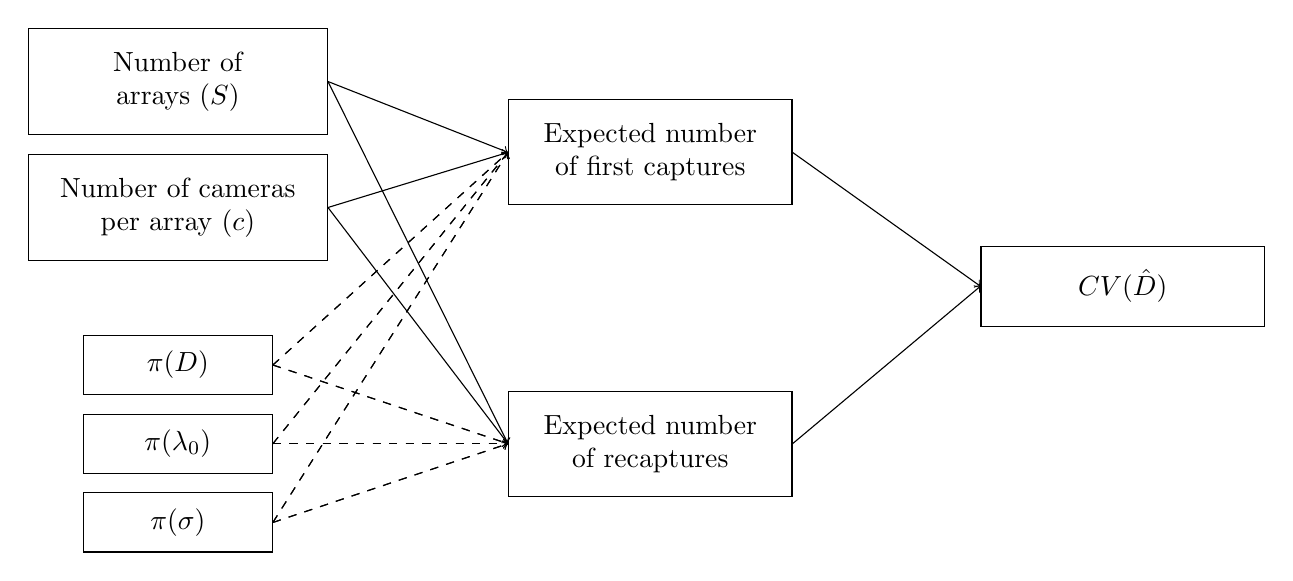
\begin{tikzpicture}[scale=2, every node/.append style={align=center,draw=black,inner sep=.3cm, minimum size=4pt, text width = 3cm}]]
  \node [text width = 3.2cm] at (0,3.3) (ar) {Number of arrays ($S$)};
  \node [text width = 3.2cm] at (0,2.5) (ca) {Number of cameras per array ($c$)};
  \node [text width = 2cm, inner sep=.2cm] at (0,1.5) (D) {$\pi(D)$};
  \node [text width = 2cm, inner sep=.2cm] at (0,1) (lam) {$\pi(\lambda_0)$};
  \node [text width = 2cm, inner sep=.2cm] at (0,0.5) (sigma) {$\pi(\sigma)$};
  \node at (3,2.85) (n) {Expected number of first captures};
  \node at (3,1) (r) {Expected number of recaptures};
  \node at (6,2) (cvd) {$CV(\hat{D})$};
  \draw[->] (ar.east) -- (n.west);
  \draw[->] (ca.east) -- (n.west);
  \draw[->] (ar.east) -- (r.west);
  \draw[->] (ca.east) -- (r.west);
  \draw[->] (n.east) -- (cvd.west);
  \draw[->] (r.east) -- (cvd.west);
    \draw[->, dashed] (D.east) -- (n.west);
  \draw[->, dashed] (D.east) -- (n.west);
      \draw[->, dashed] (lam.east) -- (n.west);
  \draw[->, dashed] (lam.east) -- (n.west);
      \draw[->, dashed] (sigma.east) -- (n.west);
  \draw[->, dashed] (sigma.east) -- (n.west);
      \draw[->, dashed] (D.east) -- (r.west);
  \draw[->, dashed] (D.east) -- (r.west);
      \draw[->, dashed] (lam.east) -- (r.west);
  \draw[->, dashed] (lam.east) -- (r.west);
      \draw[->, dashed] (sigma.east) -- (r.west);
  \draw[->, dashed] (sigma.east) -- (r.west);
\end{tikzpicture}
\label{cvd-decomp}
\caption{Large-scale camera trap design attempts to minimize $E[CV(\hat{D})]$ while remaining unbiased, by choosing values for $S$ and $c$ that offer a balance between maximizing expected number of first captures $E(n)$ (by increasing the number of arrays) and maximizing recaptures $E(r)$ (by increasing the number of cameras per array). This balance, and hence optimal choices for $S$ and $c$, are influenced by animal density and movement ($D$, $\lambda_0$, and $\sigma$), parameters of which must be estimated {\it a priori}.} 
\end{figure}

\subsection{Evaluating $CV(\hat{D})$ by simulation} \label{s:cvsim}

A possible $CV(\hat{D})$ for any candidate survey design can be calculated by selecting plausible values of the exogenous variables, simulating activity centre locations and capture histories and fitting an SECR model to those capture histories. Estimated density and its standard error are outputs of the SECR model, so $CV(\hat{D})$ can be calculated directly. As the simulation of activity centre locations and capture histories involve a random component, it is necessary to repeat the process many times, each time recording the $CV(\hat{D})$, before finally calculating the expected value of $CV(\hat{D})$ over all simulation runs. As even individual SECR models can be time-consuming to fit, evaluating $E[CV(\hat{D})]$ by simulation can take a very long time, even with parallelisation.
\\[1em]
Plausible values for $D$, $\lambda_0$, and $\sigma$ can be chosen directly, or indirectly by first specifying expected numbers of first captures and/or recaptures, and then finding values of $D$, $\lambda_0$, and $\sigma$ that return these. Since different combinations of $D$, $\lambda_0$, and $\sigma$ can return the same numbers of expected captures and recaptures, it is usually preferable to fix at least one, and preferably two, of these quantities. Often it is easier to assess plausible values for $D$ and $\sigma$, leaving only $\lambda_0$ unspecified. Analytical formulae relating $E(n)$ and $E(r)$ to $D$, $\lambda_0$, and $\sigma$ are available (see the next section). Although these expressions require numerical integration to evaluate, their availability makes it straightforward to solve for any remaining parameters using root-finding algorithms like the Newton-Raphson method.
\\[1em]
The assessment described above is only for one plausible value of each of the exogenous density and detection parameters. The distribution of simulated values of $CV(\hat{D})$ therefore reflects natural variation in $CV(\hat{D})$ arising from randomness in activity centre locations and capture histories, but does not reflect uncertainty in prior estimates of density and detection parameters. Where there is substantial uncertainty about the values these parameters might take on, which will often be the case, we recommend doing a sensitivity analysis to confirm that acceptable values of $E[CV(\hat{D})]$ are obtained across the range of plausible density and detection parameters. In principle, a distribution of simulated values of $CV(\hat{D})$ that fully reflects all uncertainties can be approximated by defining a joint prior distribution over density and detection parameters, and sampling from this distribution at the first step of each simulation run. Computation time with this approach is most likely prohibitive in most applications. Rather, we recommend first using the approximations described in the next section for exploratory analysis of potential survey and exogenous variable values. Following this, sensitivity analysis can be carried out by redoing the simulations for a few plausible combinations of exogenous parameter values. Care should be taken to include those combinations that result in relatively few recaptures (i.e.\ low, or clustered, density; small $g_0$ or $\lambda_0$; small $\sigma$), since these will generally lead to the most unfavourable values of $CV(\hat{D})$.

\subsection{Approximating $CV(\hat{D})$} \label{s:cvapprox}
Where density is uniformly distributed across the entire study area, it is possible to approximate the relationship between $CV(\hat{D})$ and $E(n)$ and $E(r)$ using results in \cite{Efford2019}: 
\begin{equation} \label{cvd}
CV(\hat{D}) \approx CF/\sqrt{\min\{E(n),E(r)\}}
\end{equation} where $CF$ is a ``correction factor'' set to 1 by default for square arrays but can be larger for more linear arrays. The approximation has no formal derivation but relies on two intuitions. The first is that natural variation in animal abundance sets an effective lower bound on how small $CV(\hat{D})$ can be, so that if the number of animals is assumed to be Poisson distributed with parameter $n$, as is commonly done, then this lower bound equals $1/\sqrt{n}$. The second is that recaptures decrease variance in $\hat{D}$. An exact relationship holds for a simple two-stage mark-recapture study. In that case, population size is estimated with the Lincoln-Petersen estimator $\hat{N}=n_1/(r/n_2)$ where $n_1$ and $n_2$ are number of captures at each visit and $r$ is number of recaptured animals that were marked. The variance of this estimator is approximated by $1/r$ \citep{Seber1982}. 
\\[1em]
The approximation in \eqref{cvd} applies a result obtained for two-stage non-spatial mark-recapture to the more general spatial capture-recapture context, but simulations reported in \cite{Efford2019} show that values of $CV(\hat{D})$ obtained by approximation closely match those obtained by simulation across a number of problem settings. Importantly, these all assume uniform density. The quality of the approximation when density varies spatially has not been established, but ignoring spatial variation in density likely leads to underestimates of $CV(\hat{D})$ \citep{Efford2019}.
\\[1em]
The expected number of first captures and recaptures can be related to design variables (number of arrays, number of cameras per array) and exogenous variables ($D$, $\lambda_0$, and $\sigma$), again using results in \cite{Efford2019}. For count detectors, and assuming a single survey occasion,
\begin{align}
E(n) &= \int_{\mathbf x} [1-\exp(-\Lambda(\mathbf x))] D(\mathbf x) d\mathbf{x} \\
E(r) &= \int_{\mathbf x} \Lambda(\mathbf x) D(\mathbf x) d\mathbf{x} - E(n)
\end{align}
where $\Lambda(\mathbf{x})=\sum_{k=1}^K \lambda(d_k(\mathbf{x}),\lambda_0,\sigma)$ is the hazard of detection (expected number of detections) at any detector for an animal with an activity centre at $\mathbf{x}$, and $\lambda(d_k(\mathbf{x}),\lambda_0,\sigma)$ is the hazard of detection at trap $k$ for an animal with an activity centre at $\mathbf{x}$. The integrals above cannot be solved in closed form, but they can be computed quickly using numerical integration. The computations are implemented in the \texttt{Enrm} function in the \texttt{secrdesign} package.

\section{Determining survey site locations} \label{s:halton}

The previous section provides methods and software for deciding how many sites to visit, and how many cameras to place, in order to achieve a desired expected level of precision in the final estimates of snow leopard density. The question remains of which sites to visit, and where to place cameras. This section addresses the first of these questions.

Estimates of density and abundance obtained using design-based inference will typically be more efficient, with lower variance, if survey points are more-or-less evenly distributed across the study region. This is because values at points close together tend to be influenced by the same underlying environmental factors and thus correlated, which increases variance. 

A survey made up of points that are more-or-less evenly distributed in space is known as spatially balanced. A regular grid of survey points is one example of a spatially balanced sample. Often, however, using a regular grid is not feasible, because some of the survey points fall in areas that are inaccessible or because the study region is highly irregular. 

Several approaches have been developed that construct grid-like designs that are flexible enough to avoid the problems that are encountered by perfectly regular grids. The most well-known methods are local pivotal methods \citep{Grafstrom2012}, generalized random tellesation stratified designs \citep{Stevens2004}, and balanced acceptance sampling \citep{Robertson2013,Vandambates2018}. We recommend and use balanced acceptance sampling, on the basis that it is easy to implement and use, and that one does not need to know the number of survey points in advance, so additional survey points can be added at any later stage while retaining good spatial balance.

Balanced acceptance sampling generates a sequence of points called a Halton sequence. The sequence is deterministic and consists of points that are evenly distributed over the interval 0-1 (Figure \ref{halton}). 

\begin{figure}[htbp]
\centering
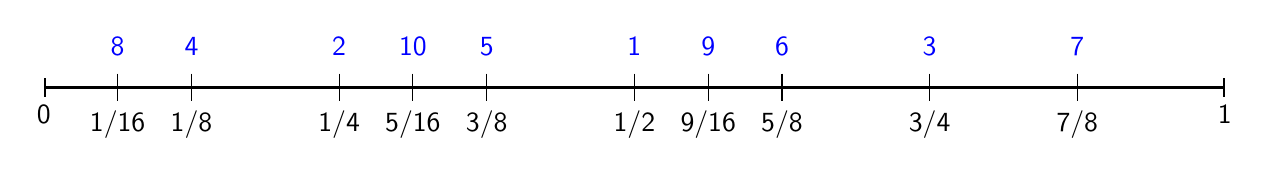
\begin{tikzpicture}[y=.0cm, x=15cm,font=\sffamily]  
  \draw[|-|,thick] (0,0)node[below=1mm]{0} -- (1,0)node[below=1mm]{1}; 
  \draw (1/2,5pt) -- (1/2,-5pt) node[anchor=north] {1/2}; 
    \draw (1/4,5pt) -- (1/4,-5pt) node[anchor=north] {1/4}; 
      \draw (3/4,5pt) -- (3/4,-5pt) node[anchor=north] {3/4}; 
      \draw (1/8,5pt) -- (1/8,-5pt) node[anchor=north] {1/8}; 
      \draw (3/8,5pt) -- (3/8,-5pt) node[anchor=north] {3/8}; 
      \draw (5/8,5pt) -- (5/8,-5pt) node[anchor=north] {5/8}; 
      \draw (7/8,5pt) -- (7/8,-5pt) node[anchor=north] {7/8}; 
      \draw (1/16,5pt) -- (1/16,-5pt) node[anchor=north] {1/16}; 
      \draw (9/16,5pt) -- (9/16,-5pt) node[anchor=north] {9/16}; 
      \draw (5/16,5pt) -- (5/16,-5pt) node[anchor=north] {5/16}; 
      
        \draw [blue] (1/2,15pt) node {1}; 
    \draw [blue] (1/4,15pt) node {2}; 
      \draw [blue] (3/4,15pt) node {3}; 
      \draw [blue] (1/8,15pt) node {4}; 
      \draw [blue] (3/8,15pt) node {5}; 
      \draw [blue] (5/8,15pt) node {6}; 
      \draw [blue] (7/8,15pt) node {7}; 
      \draw [blue] (1/16,15pt) node {8};
      \draw [blue] (9/16,15pt) node {9};  
      \draw [blue] (5/16,15pt) node {10}; 
\end{tikzpicture}
\caption{The first ten numbers in the one-dimensional Halton sequence are 1/2, 1/4, 3/4, 1/8, 5/8, 3/8, 7/8, 1/16, 9/16, 5/16. Each point is mid-way between two points generated earlier in the sequence.}
\label{halton}
\end{figure}

Two-dimensional Halton points for spatial sampling are generated using two Halton sequences, one for the $x$ dimension and one for the $y$ dimension (Figure \ref{h12}a). The key property of the Halton sequence is that not only are points evenly distributed over the whole region, they are also evenly distributed over any continuous sub-region. This has two important practical advantages. First, it allows one to start anywhere in the sequence, not necessarily at the first point, because the sequence of subsequent points will be evenly distributed no matter where one starts (Figure \ref{h12}b). This allows for an element of randomization to be introduced into the design through the selection of a random starting point. As already noted, randomization is an essential feature of a scientific design. Second, it allows additional survey points to be added whenever desired (Figure \ref{h345}a). Spatial balance is preserved in the existing survey points, new survey points, and all survey points combined. 

\begin{figure}[htbp]
\centering
  \begin{subfigure}[b]{0.45\textwidth}
    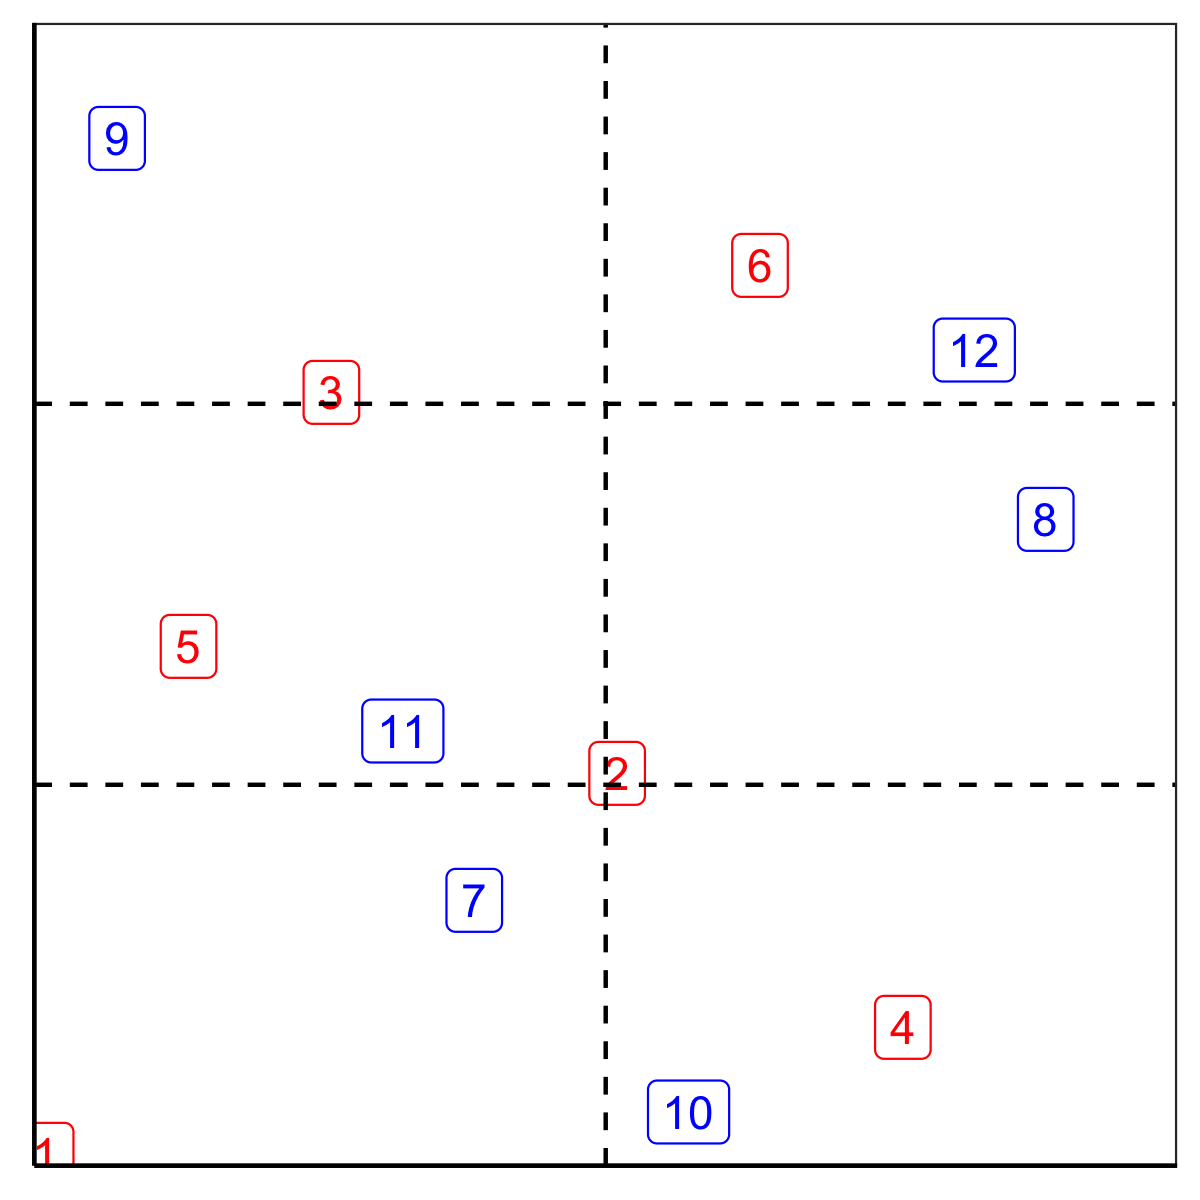
\includegraphics[width=\textwidth]{p1.png}
    \caption{}
  \end{subfigure}
  %
  \begin{subfigure}[b]{0.45\textwidth}
    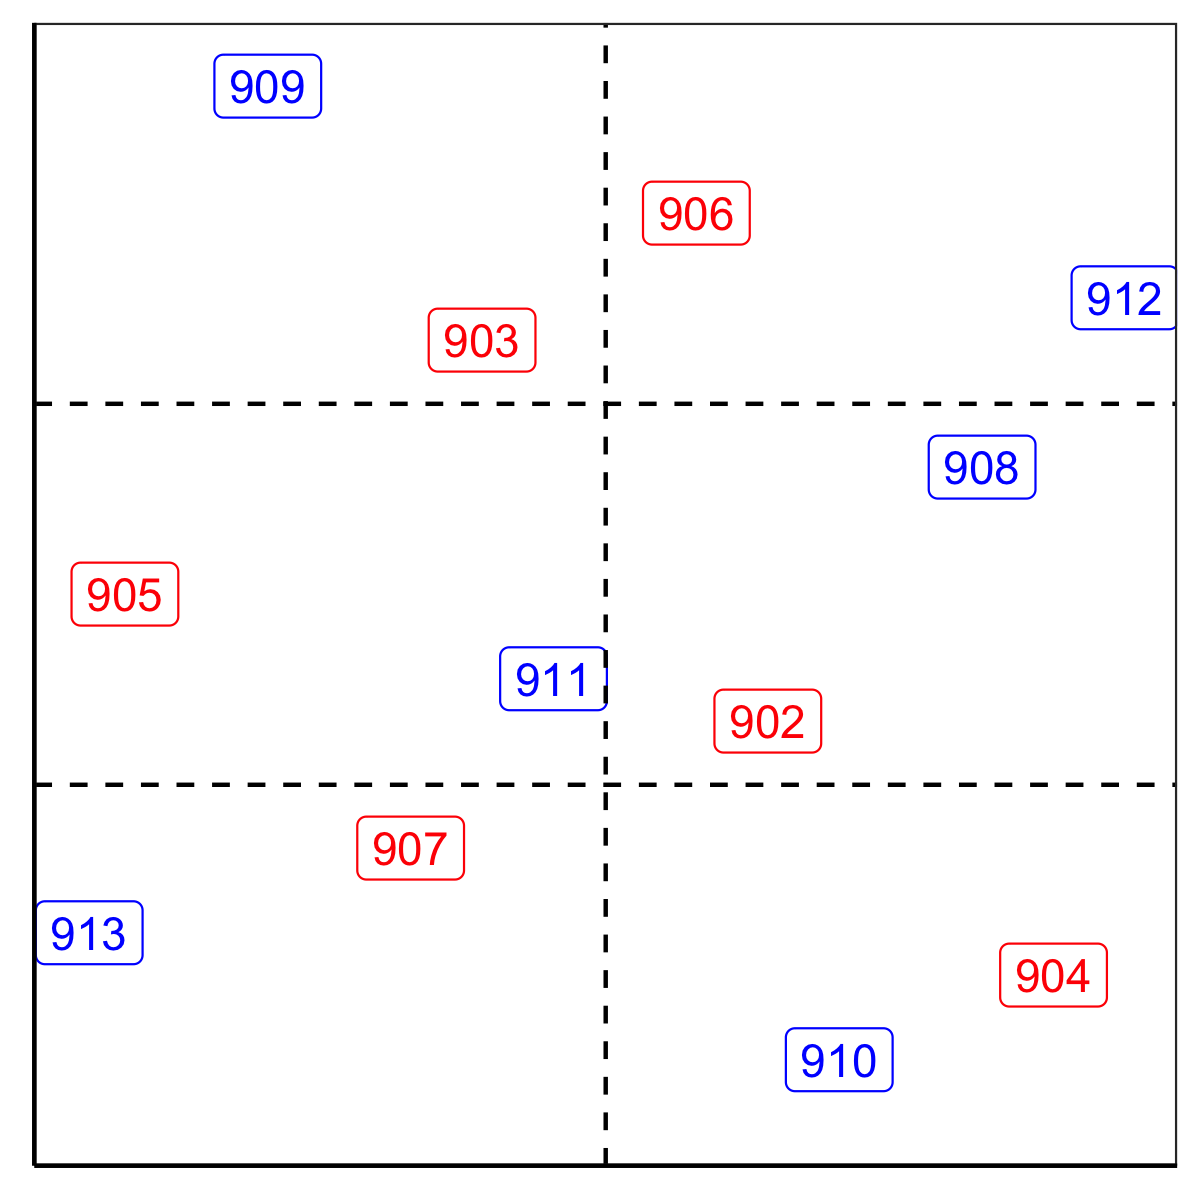
\includegraphics[width=\textwidth]{p2.png}
    \caption{}
  \end{subfigure}
\caption{Twelve two-dimensional Halton points, each representing a survey site selected by balanced acceptance sampling. Points are labelled in the order generated by the Halton sequence: 1-12 in (a), 902-913 in (b), representing two spatially well-balanced surveys generated using different random starting points. Halton sequences work by iteratively partitioning the region into smaller subregions, as shown by the dotted lines. Although the points occur in continuous space, the partition occupied by a point will not receive another point until all other partitions have also had a point added. Thus note that the first six points (shown in red) are added in a particular order that is then repeated by the second six points (shown in blue). This is the mechanism by which balanced acceptance sampling maintains spatially well-balanced points at both global and local scales.}
  \label{h12}
\end{figure}

Because balanced acceptance sampling generates a list of sequentially generated points that preserve spatial balance both overall and in smaller subregions, it is straightforward to sample areas of any shape. One simply places a minimum bounding box over the study area, and rejects any points that fall outside of the study area (Figure \ref{h345}b). Stratified sampling is done in a similar way, by taking the first $N_s$ points in the Halton sequence that fall into stratum $s$, until all samples in all strata have been generated (Figure \ref{h345}c). At any stage in the process, points remain spatially well-balanced within and across strata or within irregularly shaped study regions.

\begin{figure}[htbp]
\centering
  \begin{subfigure}[b]{0.3\textwidth}
    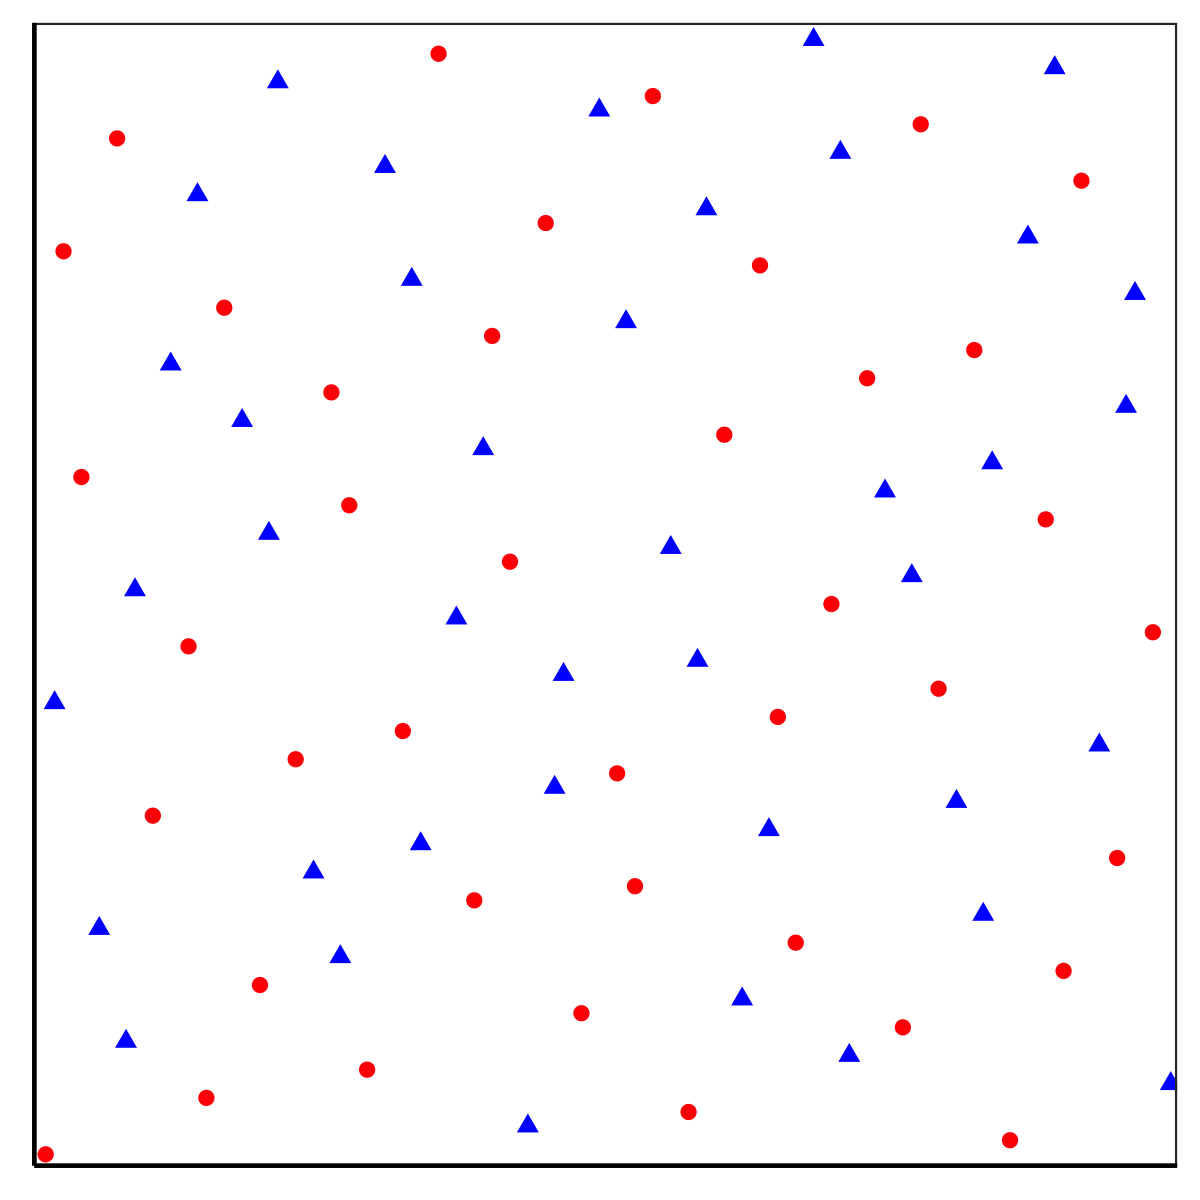
\includegraphics[width=\textwidth]{p3.png}
    \caption{}
  \end{subfigure}
  %
  \begin{subfigure}[b]{0.3\textwidth}
    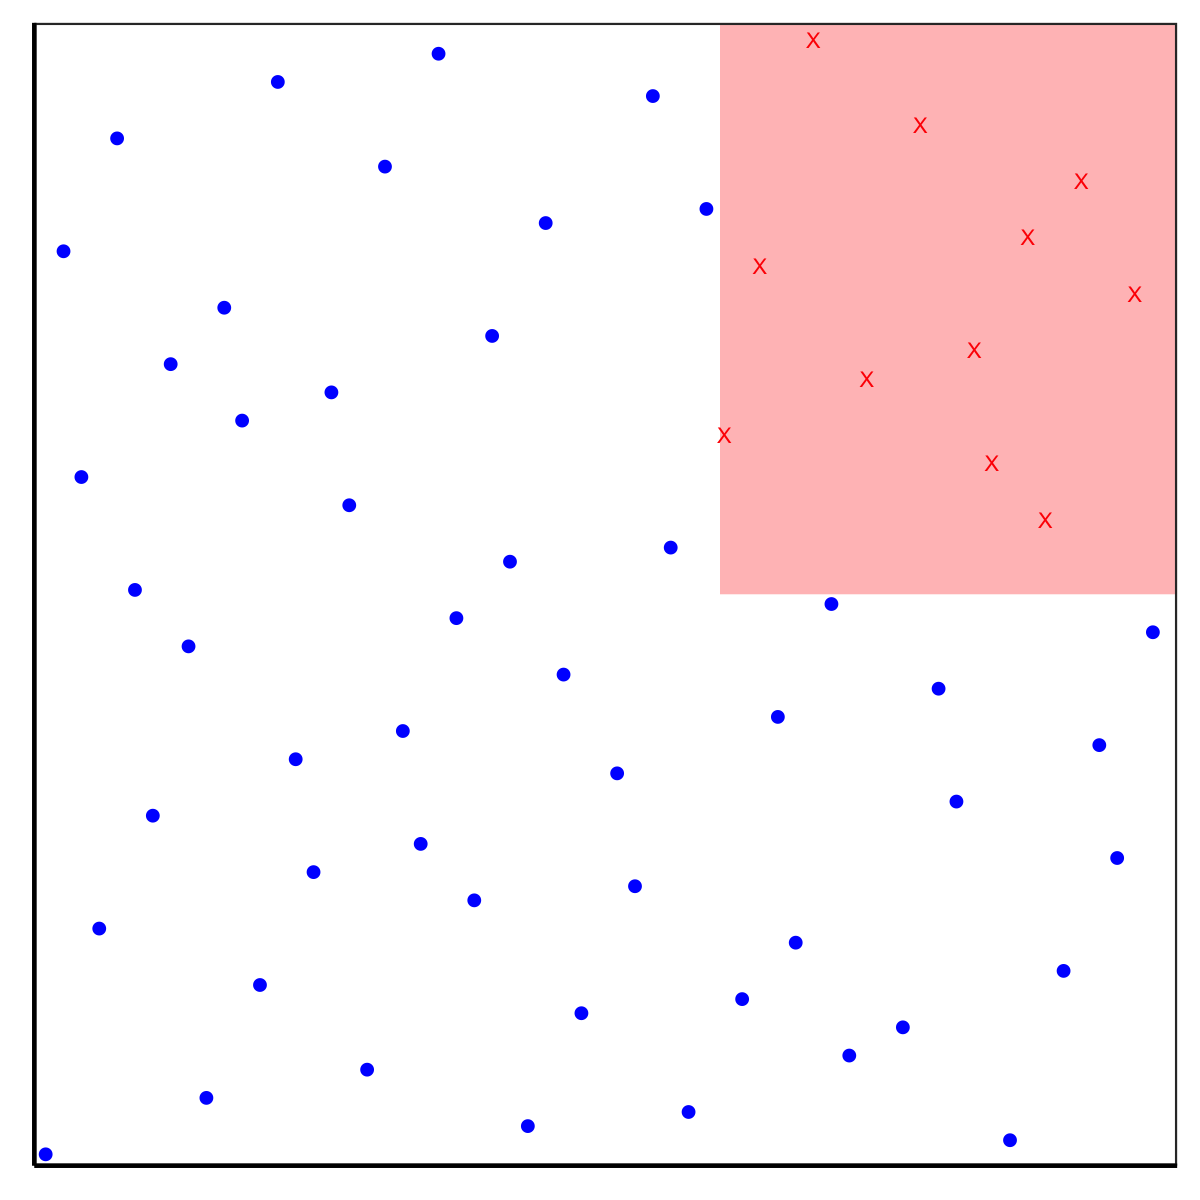
\includegraphics[width=\textwidth]{p4.png}
    \caption{}
  \end{subfigure}
    %
  \begin{subfigure}[b]{0.3\textwidth}
    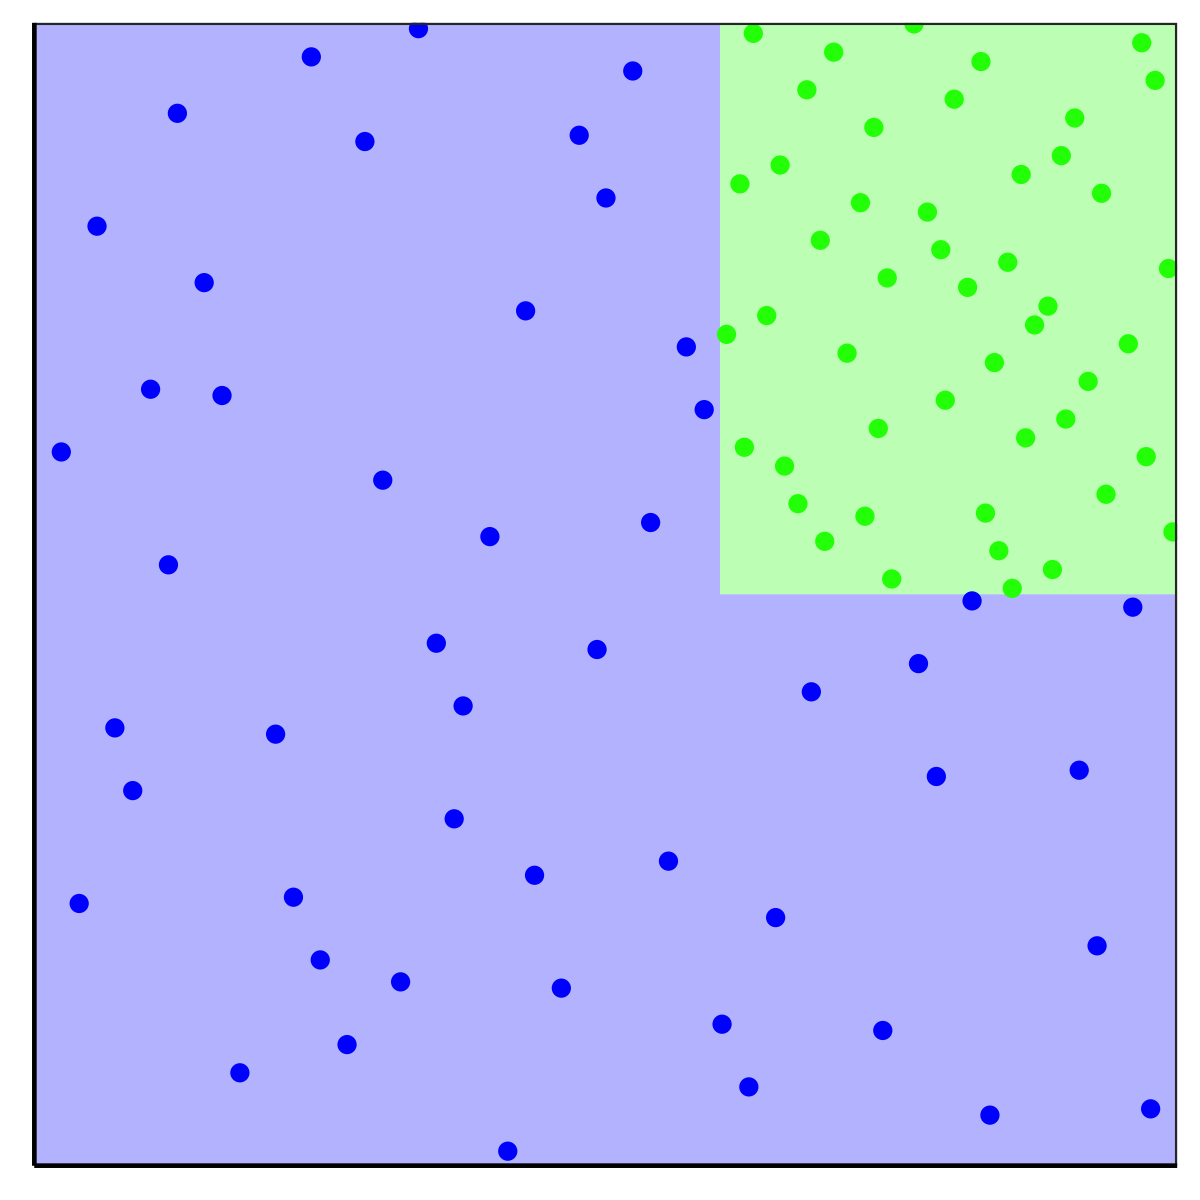
\includegraphics[width=\textwidth]{p5.png}
    \caption{}
  \end{subfigure}
  \caption{Demonstrating the key features of balanced acceptance sampling. In (a), a set of 40 new sample points (blue triangles) is added to an existing set of survey points (red circles). Both sets of points are spatially well-balanced; so is the global set of 80 points. In part (b), the red shaded area is not part of the study region, and any Halton points falling into this region are rejected. A total of 61 points were generated in order to arrive at a desired sample size of 50 points in the study region (11 rejections). In part (c) equal numbers of Halton points are generated in each of two strata, indicated by the green and blue shaded areas. Points are spatially balanced within each stratum.}
  \label{h345}
\end{figure}

Balanced acceptance sampling survey points can be generated by the following process:
\begin{enumerate}
\item Choose two random integers to indicate the starting point of the Halton sequence in each of the $x$ and $y$ dimensions.
\item Generate a large number of two-dimensional Halton points, perhaps 500 times more than the number of survey points that may be required.
\item By default, Halton points are generated to lie on the interval 0-1 in each dimension, so rescale these by the latitudinal and longitudinal extent of the survey area. 
\item If $S$ survey points are desired, select the first $S$ points in the Halton sequence that fall into the study region. In most cases, the study region will not be perfectly rectangular, and thus some of the Halton points will fall outside the study region. These points are simply rejected, and the next feasible point selected.
\end{enumerate}

By generating many more than the $S$ survey locations currently required, additional locations are kept ``in reserve'' for later use, if desired. For example, if an additional 5 survey points are desired, one simply identifies the last used point in the Halton sequence and selects the next five points in the sequence that fall into the study area. This makes it imperative that the random starting point of the Halton sequence is recorded. As Halton points require almost no computation time to generate, we recommend generating many of them. Because Halton points falling outside of the survey region are rejected, very irregularly shaped survey regions (a network of lakes, for example) require more points than regions that are close to rectangular.

\section{Supporting software}

Three R Shiny web applications have been developed to generate and evaluate candidate survey designs. One app evaluates CV by the approximation described in Section \ref{s:cvapprox}; another evaluates CV by a full Monte Carlo simulation, as described in Section \ref{s:cvsim}; and a third generates spatially balanced macro-level stratified survey designs using the approach outlined in Section \ref{s:halton}. Each app is also accompanied by an equivalent R script file that runs the same code as in the app, but without the Shiny environment. These scripts allow users to run the code line by line and provide more control to the user than the apps do. 

\subsection{Initial installation}

All apps, code, and supporting R packages are bundled together using R's \texttt{packrat} package and provided in the zip file \verb!02_paws-design.zip! submitted as an electronic appendix to the report. Both R and RStudio must be already installed. Software can be installed in two ways:
\begin{description}
\item[Using packrat (recommended)] The way requires that the \texttt{packrat} R package is installed, but otherwise takes care of any other packages that need to be installed. Packrat installs packages locally, so any packages installed here will not interfere with any other versions of packages you have already installed. Steps involved are:
\begin{enumerate}
\item Open RStudio and load the packrat library with \verb!library(packrat)!
\item Recreate the project library with \verb!packrat::unbundle(bundle, where)!, where \texttt{bundle} is the path to the zip file (between quotes) and \texttt{where} is the directory where the project will go (also in quotes, and this directory must already exist). For example, if the zip file is saved to a directory \verb!\Documents! and the project should be extracted to the directory \verb!\Documents\PAWS! then type the following into the command line: \verb!packrat::unbundle(''~\Documents'', ''~\Documents\PAWS''!. These paths will differ depending on the operating system used. Unbundling the project will take several minutes as all packages need to be downloaded and installed.  
\item If everything has worked you should be able to browse to the project directory and open the project by clicking on the project file \texttt{macro-design.Rproj}, and then run any of the apps or script files located in the project subfolders. 
\item If the apps and/or script files give errors it might be necessary to manually install the required packages. First try doing this using \texttt{packrat} by typing \verb!packrat::status()! and then \verb!packrat::restore()! at the command line. Some R packages require external (non-R) libraries to be installed and if these are not available this will have to be done manually before repeating this step until all packages have been successfully installed. One error that seems to arise quite often relates to the library \verb!cairo!. This can be installed in mac OSX by \verb!brew install cairo! and in ubuntu using \verb!sudo apt-get install libcairo2-dev libjpeg-dev libgif-dev! (at the terminal).
\item If all else fails, try the other method described below.
\end{enumerate}
\item[Manual package installation] This way requires manually installing each of the R packages required by the apps and scripts. These packages will be installed into your main R package library. Steps involved are:
\begin{enumerate}
\item Unzip the zip file \verb!02_paws-design.zip! to a folder. Delete the subfolder called \texttt{packrat} and all its contents. 
\item Open RStudio and open the project file \texttt{macro-design.Rproj}.
\item Install the required packages by pasting the following into the console
\\[1em]
\texttt{install.packages("shiny")} \\
\texttt{install.packages("dplyr")} \\
\texttt{install.packages("ggplot2")} \\
\texttt{install.packages("plotly")} \\
\texttt{install.packages("secrdesign")} \\
\texttt{install.packages("viridis")} \\
\texttt{install.packages("tidyr")} \\
\texttt{install.packages("purrr")} \\
\texttt{install.packages("sf")} \\
\texttt{install.packages("mapview")} \\
\texttt{install.packages("leaflet")} \\
\texttt{install.packages("htmltools")} \\
\texttt{install.packages("raster")} \\
\texttt{install.packages("secr")} \\
\texttt{install.packages("secrdesign")} \\
\texttt{install.packages("readr")} \\
\texttt{install.packages("BalancedSampling")} 
\end{enumerate}
\end{description}

\subsection{Software for fast approximate evaluations of $CV(\hat{D})$}

\subsubsection{Starting the app}
Open the R project by clicking on \texttt{macro-design.Rproj}. Then browse to the \textit{cv-fast-approx} folder, select the \texttt{app.R} file in that folder, and click the \textit{Run app} button. 

\subsubsection{Running the app}

\begin{enumerate}
\item CV calculations require the user to first enter the following information in the left-hand toolbar (Figure \ref{cva-1}):
\begin{enumerate}
\item A range of values for possible number of survey sites, using the slider bar titled \textit{Number of sites}. Note that this refers the number of study regions or areas, not the number of cameras, which is set using the following slider.
\item A range of values for possible number of cameras to be used at each site, using the slider bar titled \textit{Number of cameras per site}. Note that each site uses the same number of cameras, with the number of cameras at each site varied as part of the simulation.
\item Snow leopard density ($\pi(D)$) per 100km$^2$, in the box titled \textit{Expected D/100km2};
\item The intensity of detections at the activity center ($\pi(\lambda_0))$, in the box titled \textit{Expected lambda};
\item The rate at which intensity decreases with distance from the activity center ($\pi(\sigma)$), in the box titled \textit{Expected sigma}. 
\item The distance between camera traps, expressed as a multiple of the value in the \textit{Expected sigma} box, in the box entitled \textit{Trap spacing (multiple of sigma)}.
\item A ``correction factor'' that serves to increase the CV for extra-Poisson variation in density (or other non-idealities in the survey process). Approximations of CV assume constant animal density and optimal (square) grids of camera traps, and likely underestimate CV when density is non-uniform or other non-idealities are present. This is an experimental feature and it is not clear what values are most appropriate, but values between 1 (no change) and 2 are suggested. The rationale for this is that, under the constant density assumption, the mean and variance of the number of activity centres per unit area are equal (by standard properties of Poisson processes). Design of distance sampling surveys have incorporated extra-Poisson variation by a multiple of 3 i.e.\ variance is three times the mean. 
\end{enumerate}
\item Once values for these have been selected CV is calculated by clicking the ``Calculate CV'' button. CV results are presented in the form of a figure such as the one shown in Figure \ref{cva-1}. Colours represent CV values for various combinations of number of sites (horizontal axis) and numbers of cameras per site (vertical axis), with darker colours indicating higher (i.e.\ worse) CVs. A red contour line indicates a CV of 30\%, the minimum acceptable CV for the PAWS project. A second, blue contour line indicates a CV of 20\%. A user can hover over individual cells on the surface to display a pop-up box containing information on the expected number of first captures (unique animals), recaptures, and the precise CV achieved from these.
\end{enumerate}

\begin{figure}[htbp]
\centering
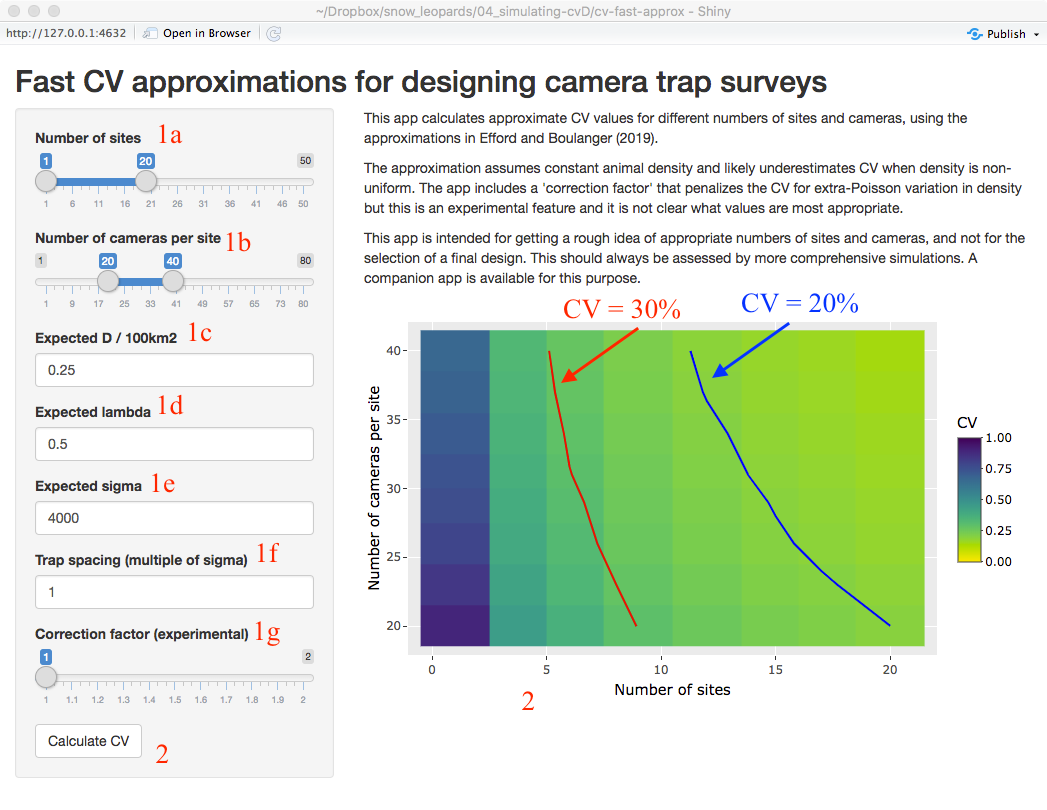
\includegraphics[width=\textwidth]{cv-approx-1}
\caption{Screenshot of software for fast approximate evaluations of $CV(\hat{D})$. Users enter input data on key design variables in the left-hand toolbar, and then click ``Calculate CV'' to generate the main plot, which shows how $CV(\hat{D})$ varies with survey effort. Note that this approximate calculation of $CV(\hat{D})$ relies on some strong simplifying assumptions, and so any final checks of CV should also use the full simulation approach described in the next section.}
\label{cva-1}
\end{figure} 

\subsection{Software for evaluating $CV(\hat{D})$ by simulation}
This app is intended to be a comprehensive evaluation of the expected CV under a completely specified survey design, meaning all camera trap locations must be provided, and the survey region must be defined. Multiple independent surveys can be included if desired. The user then needs to specify details of the processes generating animal activity centres and determining the scale of animal movement. In contrast to the previous app, users have much more control over these processes. For example, density can depend on spatial covariates (including latitude and longitude) and movement can incorporate non-Euclidean distances. In cases of multiple surveys, these details can vary by survey region. Once specified, the app simulates a desired number of capture histories, which should be inspected to check that roughly appropriate numbers of first captures and recaptures have been simulated. Finally, SCR models are fitted to each of the simulated capture histories and expected CV results obtained by averaging over simulation runs. If multiple survey regions are used, expected CVs are generated for abundance estimates within each region as well as over the entire area consisting of all survey regions.

\subsubsection{Starting the app}
Open the R project by clicking on \texttt{macro-design.Rproj}. Then browse to the \textit{cv-full-sim} folder, select the \texttt{app.R} file in that folder, and click the \textit{Run app} button. 

\subsubsection{Running the app}

\begin{enumerate}
\item Prepare and load \texttt{.Rds} files containing study area meshes and camera trap locations. These should be in UTM coordinates. The UTM zone is automatically inferred from the centre of the displayed map, so before loading the meshes and trap locations the centre of the map should be placed at the rough centre of the study area. Otherwise, the projection string will need to be entered into the source code used to generate the app. Use the ``Browse'' buttons to select files containing:
\begin{enumerate}
\item \textit{File for traps}. For a single study region, a data frame with two columns $x$ and $y$ containing the locations of all camera traps. For multiple study regions, a {\it list} in which each element of the list contains a data frame for a study region. The specified file must be in \texttt{.Rds} format.
\item \textit{File for meshes}. For a single study region, a mesh as used in the \texttt{secr} package. For multiple study regions, a {\it list} in which each element of the list contains a mesh for a study region. The specified file must be in \texttt{.Rds} format.
\end{enumerate}
Fine-scale meshes can slow down the app dramatically and often the resolution of the mesh can be reduced without materially affecting results. The \textit{Reduce mesh size} check box reduces the resolution of the mesh by a factor of three and can be used if the app is very slow or for exploratory types of analyses. Sensitivity checks should always be run to determine the effect of any reduction in mesh resolution.
\item Select the desired number of simulations to run, in \textit{Simulations to run}. Note that fitting SCR models can be very time consuming, so the ``Run SCR'' part of the analysis may take several hours or even days if a large number of simulation (say 100) are used. Our recommendation is to start with just a few simulations to check that everything is running correctly. Then, run 10 simulations and see how variable results are over simulations. If CV does not vary much then a large number of simulations is not needed. Depending on how much CV varies from simulation to simulation, a final run of 50-100 simulations can then be implemented to collect the final results.
\item Enter suitable values for parameters affecting the density of animal activity centres:
\begin{enumerate}
\item Mean snow leopard density ($\pi(D)$) per 100km$^2$, in the box titled \textit{Expected D/100km2};
\item If density varies spatially, then the name of a covariate on which density depends, in the {\it Name of density covariate} box. Note that this variable name must appear as a mesh covariate in the mesh file specified earlier. If the goal is simply to investigate the effects of non-uniform density, then either longitude ($x$) or latitude ($y$) can be entered as covariate names. Only one covariate is allowed. For uniform density this box can be ignored.
\item The strength of the relationship between the density covariate and animal density, in the {\it Coeff. of density covariate} box. This value is the coefficient associated with the spatial covariate in the linear predictor used to construct animal density (using, by default, a log link). For uniform density across the study region this value should be zero. Densities are rescaled so that the mean density over the survey area is equal to that given in the \textit{Expected D/100km2} box.
\end{enumerate}
\item Enter suitable values for parameters affecting the detection process (or equivalently, the movement of animals around their activity centres):
\begin{enumerate}
\item The intensity of detections at the activity center ($\pi(\lambda_0)$, in the box titled \textit{Expected lambda};
\item The rate at which intensity decreases with distance from the activity center ($\pi(\sigma)$), in the box titled \textit{Expected sigma};
\item If detection is affected by covariates other than the Euclidean distance between an animal's activity centre and a camera trap, then the name of the covariate affecting animal conductance can be specified in the {\it Name of conductance covariate} box. Note that this variable name must appear as a mesh covariate in the mesh file specified earlier. Only one covariate is allowed. If non-Euclidean distances are not required i.e.\ if the conventional Euclidean distance suffices, then this box can be ignored.
\item The strength of the relationship between the conductance covariate and animal conductance, in the {\it Coeff. of density covariate} box. This value is the coefficient associated with the spatial covariate in the linear predictor used to construct the ``noneuc'' variable in package \texttt{secr} (using, by default, a log link). The ``noneuc'' variable is then used to construct conductances between points and shortest path distances (see \cite{Sutherland2015} for details). If conventional Euclidean distance is to be used then this value should be zero. 
\end{enumerate}
\item Different base maps can be displayed by selecting from the \textit{Base map} drop-down menu (Figure \ref{mac-2345}). The three current options are \textit{OpenStreetMap}, a basic map of major geographical features and points of interest; \textit{EsriWorldImagery}, a detailed satellite map showing topography, and \textit{EsriWorldStreetMap}, which is similar to \textit{OpenStreetMap} but also displays topography (set as default).  
\item Click the ``Add region'' button. This displays the trap and mesh objects specified in the \textit{File for traps} and \textit{File for meshes} files on the map, and associates them with the set of density and movement parameters just entered. Further survey regions, each with their own set of traps and other exogenous parameter values, can be added by repeating the steps above. Note that if the file uploaded using \textit{File for traps} and \textit{File for meshes} contains multiple areas then {\it all} of those areas are allocated the same exogenous parameter values (those appearing at the time that the ``Add region'' button is clicked).
\item Click the ``Simulate histories'' button. This simulates the desired number of capture histories. A summary table is displayed in the top right hand part of the screen showing the min-max range of first sightings (\textit{N.animals}) and recaptures (\textit{N.recaps}) across simulations. These should be inspected to check that they are appropriate i.e.\ are roughly in line with how many captures and recaptures are expected to occur. 
\item Click the ``Run SCR'' button. This fits a constant density SCR model to each of the simulated capture histories and extracts two estimates of animal abundance from each -- {\it expected} abundance $\hat{N}_e$ and {\it realised} abundance $\hat{N}_r$. Realised abundance is the sum of animals actually detected by the survey and the expected number of animals not detected. It takes into account only uncertainty in the number of undetected animals, which is appropriate when the goal is to estimate how many animals currently occupy the survey area, but not appropriate where the goal is to extrapolate beyond the survey area, as is the goal with PAWS surveys. In that case it is important to use expected abundance, which is the sum of the number of animals {\it expected} to be detected by the survey and the expected number of non-detected animals. This measure takes into account uncertainty about both detected and non-detected animals and, for this reasons, variances and CVs for expected abundance will tend to be larger than for realised abundance. The difference between expected and realised CVs tends to be small when a relatively small proportion of a study area is covered by camera traps, because the number of undetected animals dominates and both CVs take this uncertainty into account, but large differences can emerge when survey coverage is high. A summary table is displayed below the capture history table showing the expected CV of expected animal abundance \verb!CV_E.N! and the expected CV of realised animal abundance \verb!CV_R.N!. Results are shown in each region, as well as pooled over all regions. 
\item All model output returned by the \texttt{secr.fit} function in the \texttt{secr} package can be downloaded (together with the model meshes, traps objects, and capture histories) using the ``Download all'' button at the bottom left of the screen. All capture history output returned by the \texttt{sim.capthist} function in the \texttt{secr} package can be downloaded (together with the model meshes and traps objects) using the ``Download capthists'' button at the bottom left of the screen (this is useful for inspecting the capture histories before running SCR models).
\end{enumerate}

\begin{figure}[htbp]
\centering
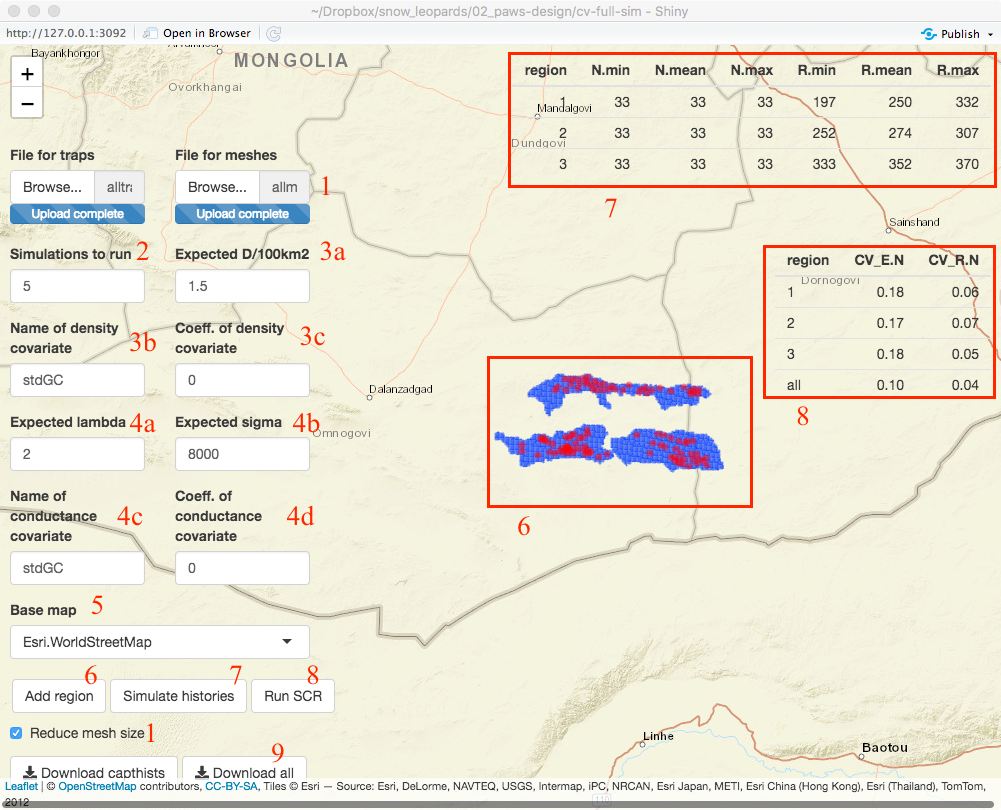
\includegraphics[width=\textwidth]{cv-full}
\caption{Screenshot of software for comprehensive evaluations of $CV(\hat{D})$ by Monte Carlo simulation. Users again enter input data on key design variables in the left-hand toolbar, although here there is greater flexibility in the kinds of density and detection processes that can be modelled (for example, non-uniform density and non-Euclidean animal movement). Given these inputs, the app simulates a set of capture histories and fits a constant density SCR model to each of these. Expected CV results for expected abundance/density (appropriate for extrapolation beyond the survey area; recommended for PAWS surveys) and realised abundance/density (appropriate when the scope is limited to the study area; not recommended) are extracted from these fitted models. The screenshot illustrates the application of the software to assess the expected CV of an actual study conducted over three survey regions in Mongolia.}
\label{cva-1}
\end{figure} 

\subsection{Software for generating survey site locations}

\subsubsection{Starting the app}
Open the R project by clicking on \texttt{macro-design.Rproj}. Then browse to the \textit{generate-macro-sites} folder, select the \texttt{app.R} file in that folder, and click the \textit{Run app} button. 

\subsubsection{Preparing and loading study area shape files}
Input data for the app consists of a set of shape files demarcating the study area. A stratification variable must be added to the shape file prior to using the app. This variable must be called \texttt{stratum}, and identifies the stratum that each raster grid cell belongs to. It should be a factor variable; if the variable is numeric (e.g.\ if numbers have been used to label strata) it will be coerced to a factor variable. If there is no variable called \texttt{stratum} in the shape file the app will return an error.

The user selects the shape file input by clicking the ``Browse'' button located next to ``Load new survey area'' and selects the survey area shape files. Note that a shape file consists of four files -- a \texttt{.dbf}, \texttt{.prj}, \texttt{.shp}, and \texttt{.shx} file -- and all four of these must be selected at the same time. Once files have been loaded, the app plots the study area, with strata shown in red/orange/yellow, and zooms to the extent of the study area (Figure \ref{mac-1}). 

\begin{figure}[htbp]
\centering
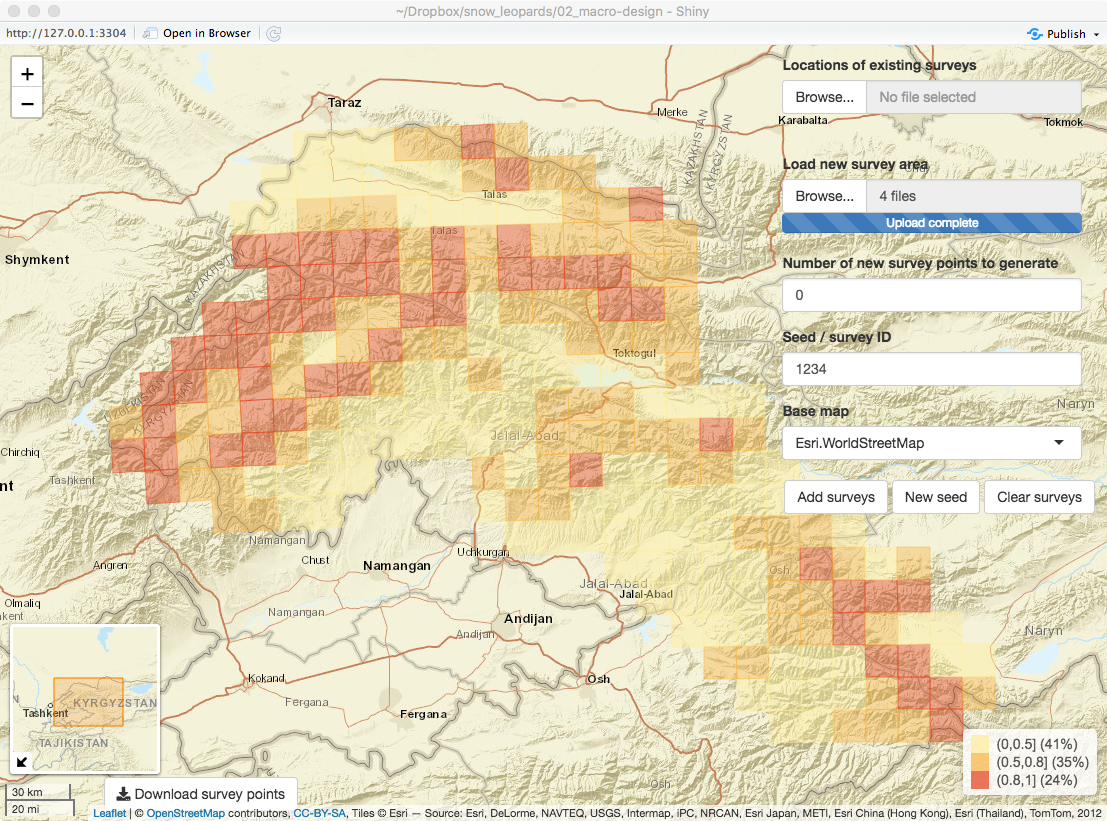
\includegraphics[width=\textwidth]{mac-1}
\caption{Screenshot of software for generating survey site locations, once a shape file defining the study area and any stratifying variable has been uploaded. Here the study region has been stratified by predicted snow leopard occupancy probabilities (yellow = low, red = high). The legend in the bottom right of the screen shows the cutoffs used in the stratification and the proportion of survey effort allocated to each stratum. These can be changed by editing the code used to generate the app.}
\label{mac-1}
\end{figure}

Users can zoom in and out using the + and -- buttons or using the mouse scroller to investigate the study area (Figure \ref{mac-2345}a-b). Different base maps can be displayed by selecting from the \textit{Base map} drop-down menu (Figure \ref{mac-2345}c-d). The three current options are \textit{OpenStreetMap}, a basic map of major geographical features and points of interest; \textit{EsriWorldImagery}, a detailed satellite map showing topography, and \textit{EsriWorldStreetMap}, which is similar to \textit{OpenStreetMap} but also displays topography (set as default).  

\begin{figure}[htbp]
\centering
  \begin{subfigure}[b]{0.49\textwidth}
    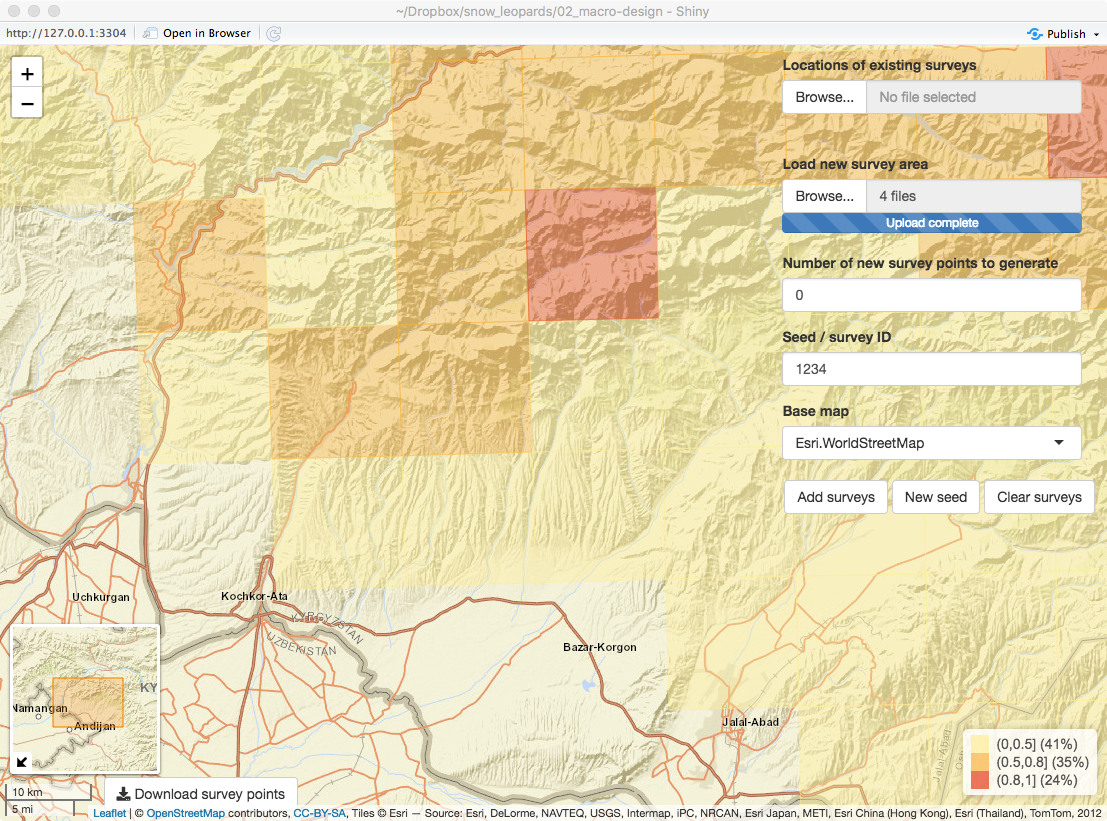
\includegraphics[width=\textwidth]{mac-2}
    \caption{}
  \end{subfigure}
  %
  \begin{subfigure}[b]{0.49\textwidth}
    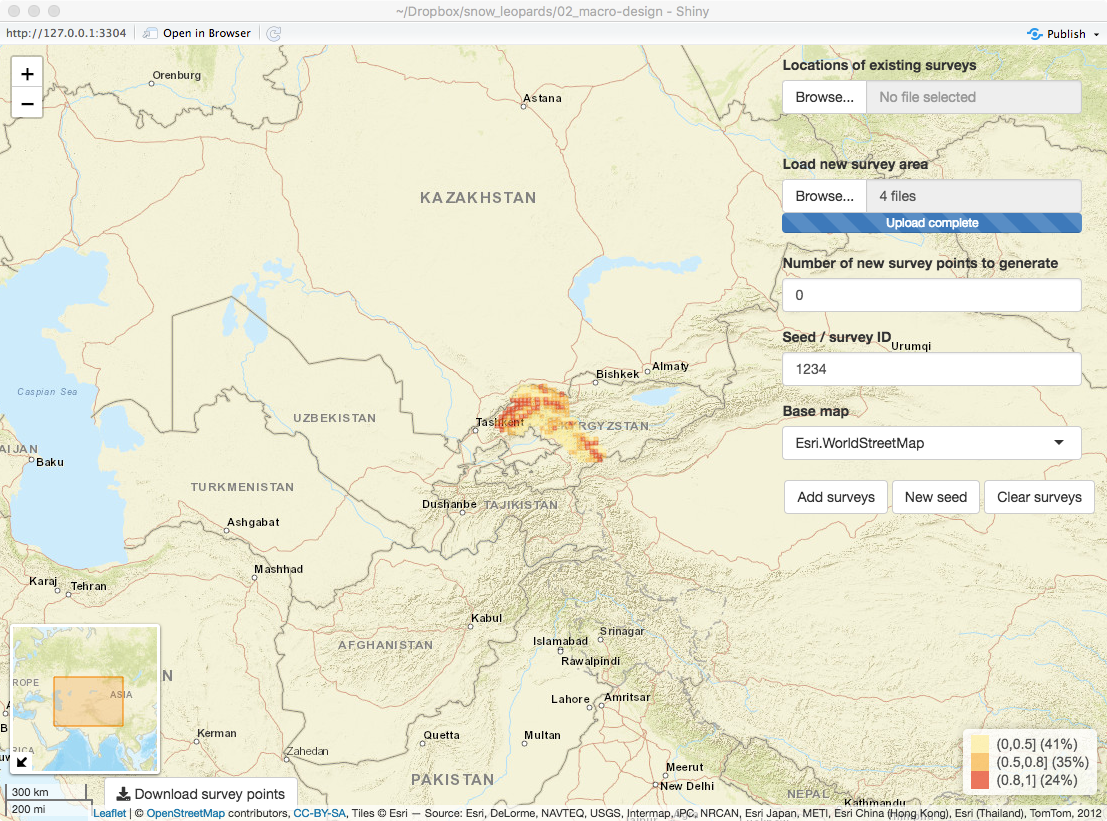
\includegraphics[width=\textwidth]{mac-3}
    \caption{}
  \end{subfigure} \\
    \begin{subfigure}[b]{0.49\textwidth}
    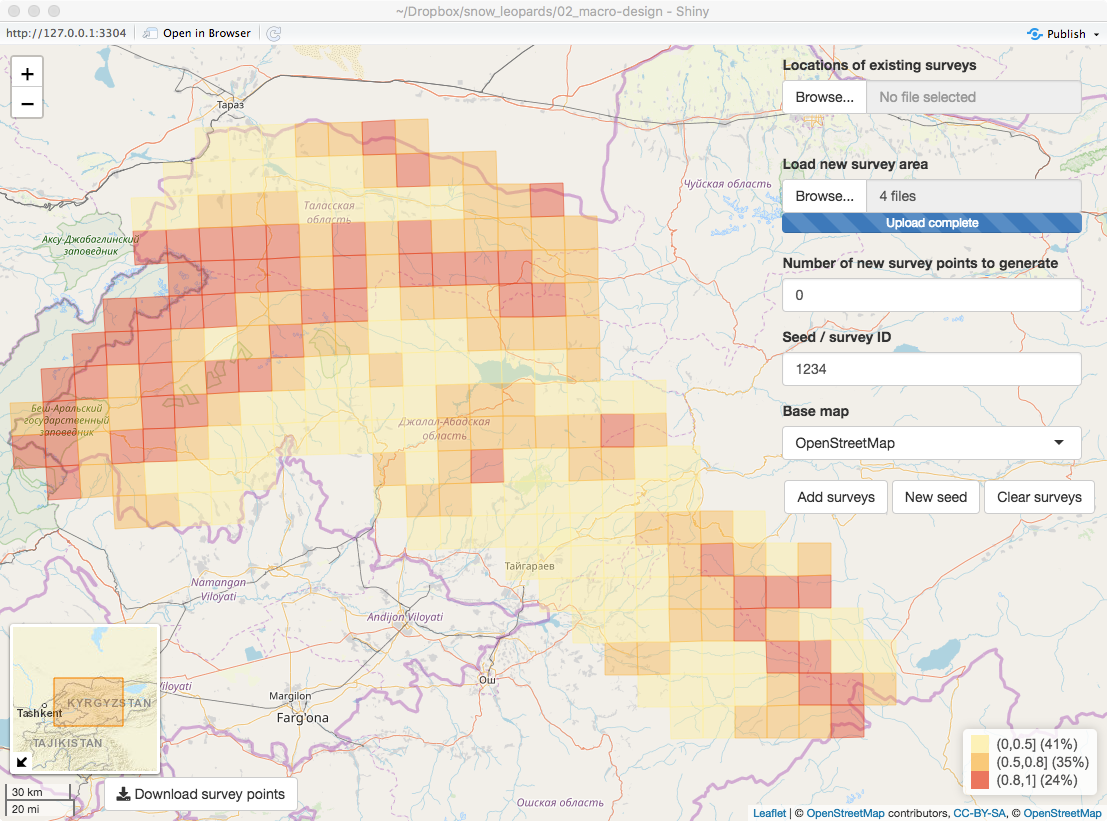
\includegraphics[width=\textwidth]{mac-4}
    \caption{}
  \end{subfigure}
  %
  \begin{subfigure}[b]{0.49\textwidth}
    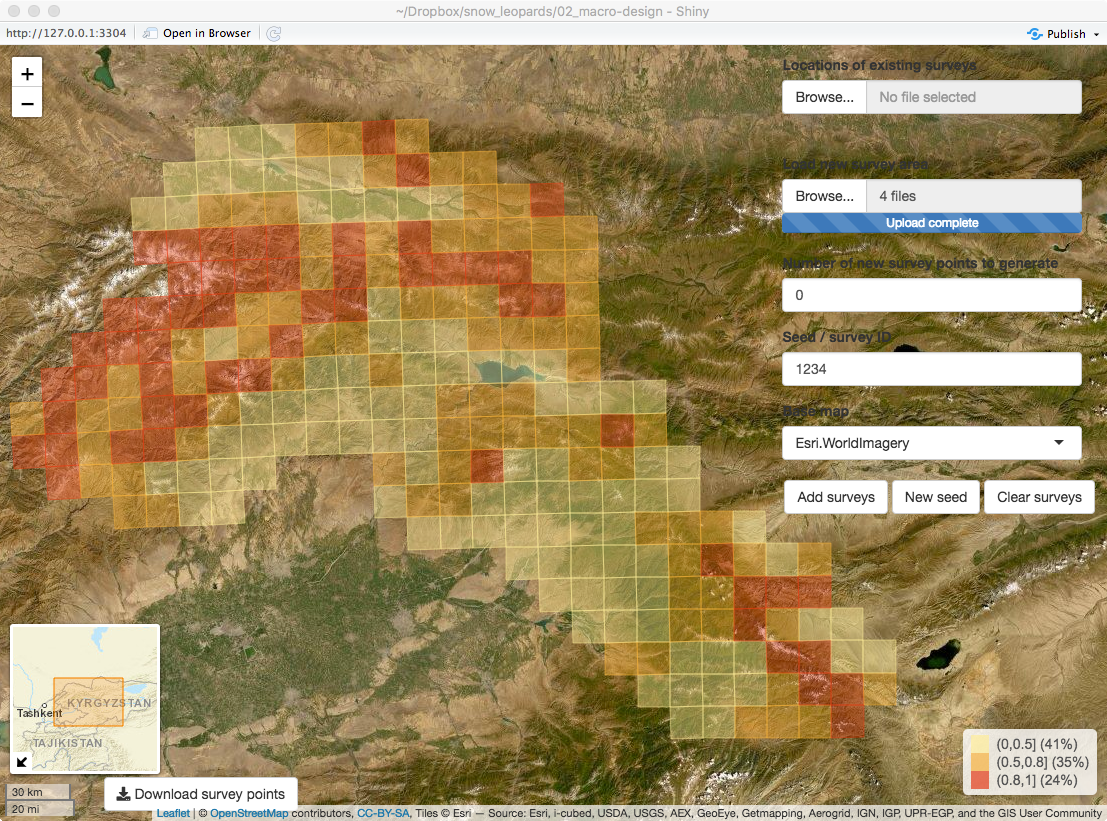
\includegraphics[width=\textwidth]{mac-5}
    \caption{}
  \end{subfigure}
\caption{The map used in the software is interactive, and users can (a) zoom in and (b) zoom out to investigate the study area, and can display different aspects of the region through the choice of different base maps (current options are (c) \textit{OpenStreetMap}, (d) \textit{EsriWorldImagery}, and the default option (a,b) \textit{EsriWorldStreetMap})}
\label{mac-2345}
\end{figure}

Once the shape files have been added, a legend appears in the bottom right hand corner showing the strata labels and the proportion of survey points to be generated from each stratum in brackets. These should be carefully checked to make sure they reflect the desired properties of the design. 

The proportion of points generated in each stratum default to the relative area covered by the stratum (area-proportional sampling). This means that a stratum covering twice the area of another will receive twice as many survey points; or that each cell in the survey area has equal inclusion probability. These proportions can be changed, but only by accessing the code used to generate the app. This should only be done in consultation with a statistician.

\subsubsection{Excluding areas already sampled}
As described in the previous section, one option to avoid sampling in areas that have already been sampled is simply to reject any survey points that fall into these areas. This is most easily done by examining the set of survey points generated, assessing how many points are to be rejected, and generating that many additional points, repeating this process until the desired number of survey points has been achieved. 

Another option is to load the masks associated with existing surveys, in which case no points will be generated in the areas covered by the mask. This can be done by setting up a \texttt{.rds} file containing a list of mask objects, one for each previous survey. This file can be loaded into the app via the \textit{Browse} button next to \textit{Locations of existing surveys}. The areas already surveyed will appear as grey polygons plotted on top of the existing grid (Figure \ref{mac-6789}a). No survey points will be generated inside these areas. 

\begin{figure}[htbp]
\centering
  \begin{subfigure}[b]{0.49\textwidth}
    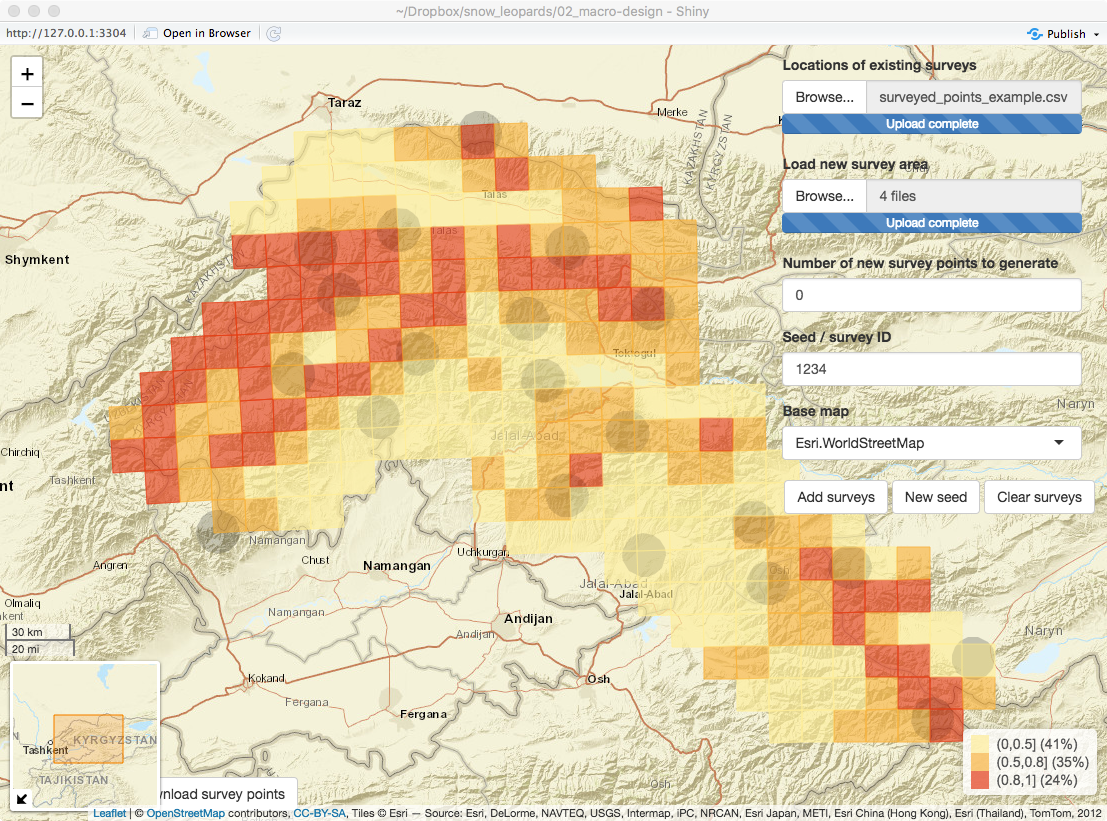
\includegraphics[width=\textwidth]{mac-6}
    \caption{Excluding already sampled areas}
  \end{subfigure}
  %
  \begin{subfigure}[b]{0.49\textwidth}
    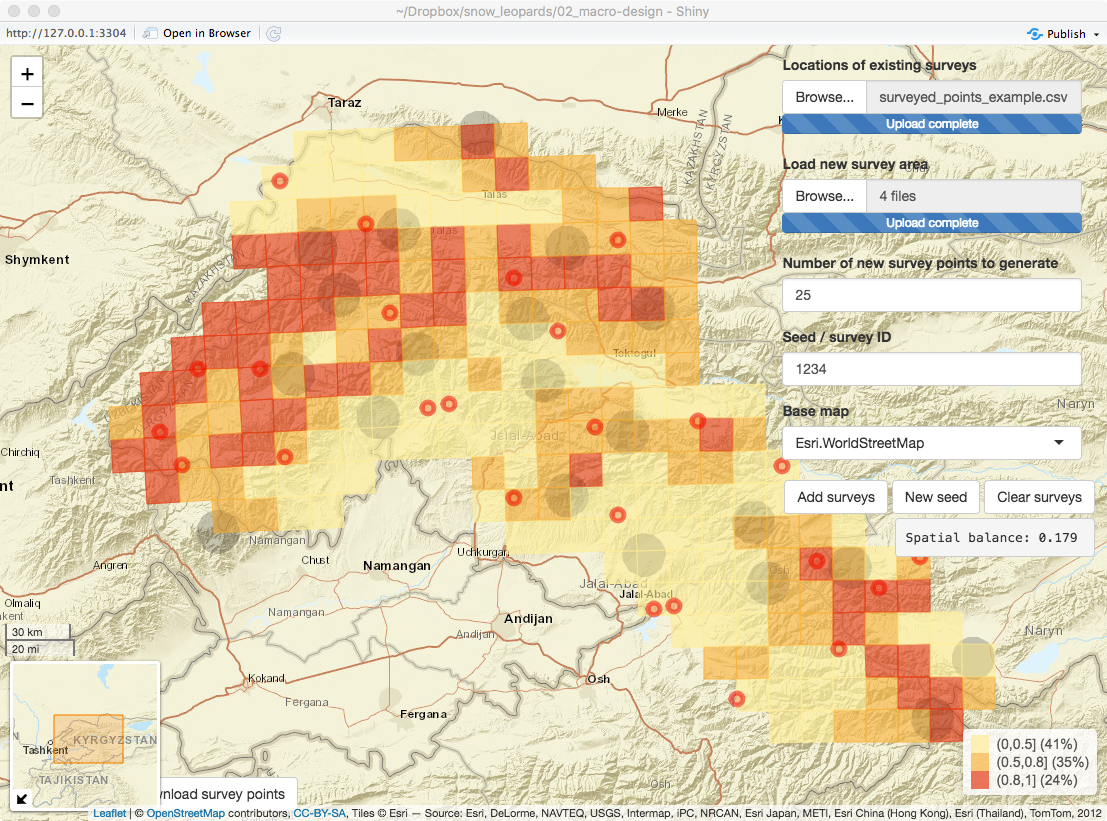
\includegraphics[width=\textwidth]{mac-7}
    \caption{Adding 25 survey points}
  \end{subfigure} \\
    \begin{subfigure}[b]{0.49\textwidth}
    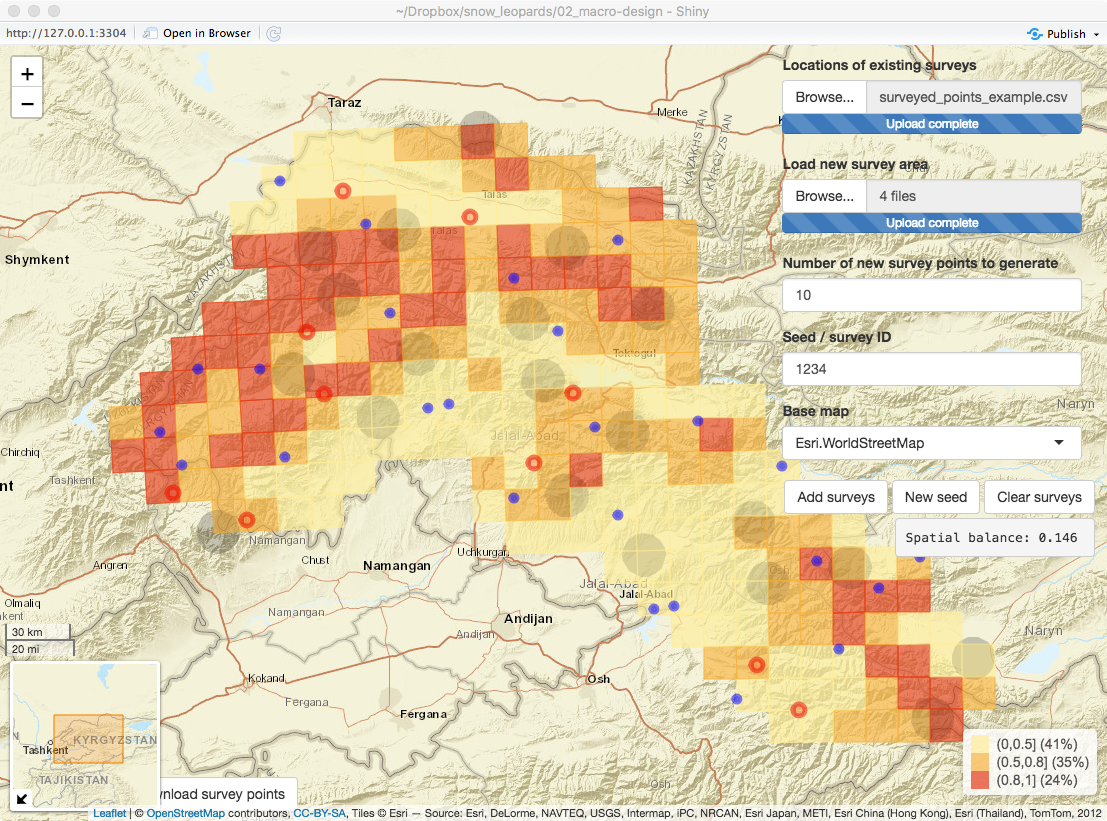
\includegraphics[width=\textwidth]{mac-8}
    \caption{Adding an additional 10 survey points}
  \end{subfigure}
  %
  \begin{subfigure}[b]{0.49\textwidth}
    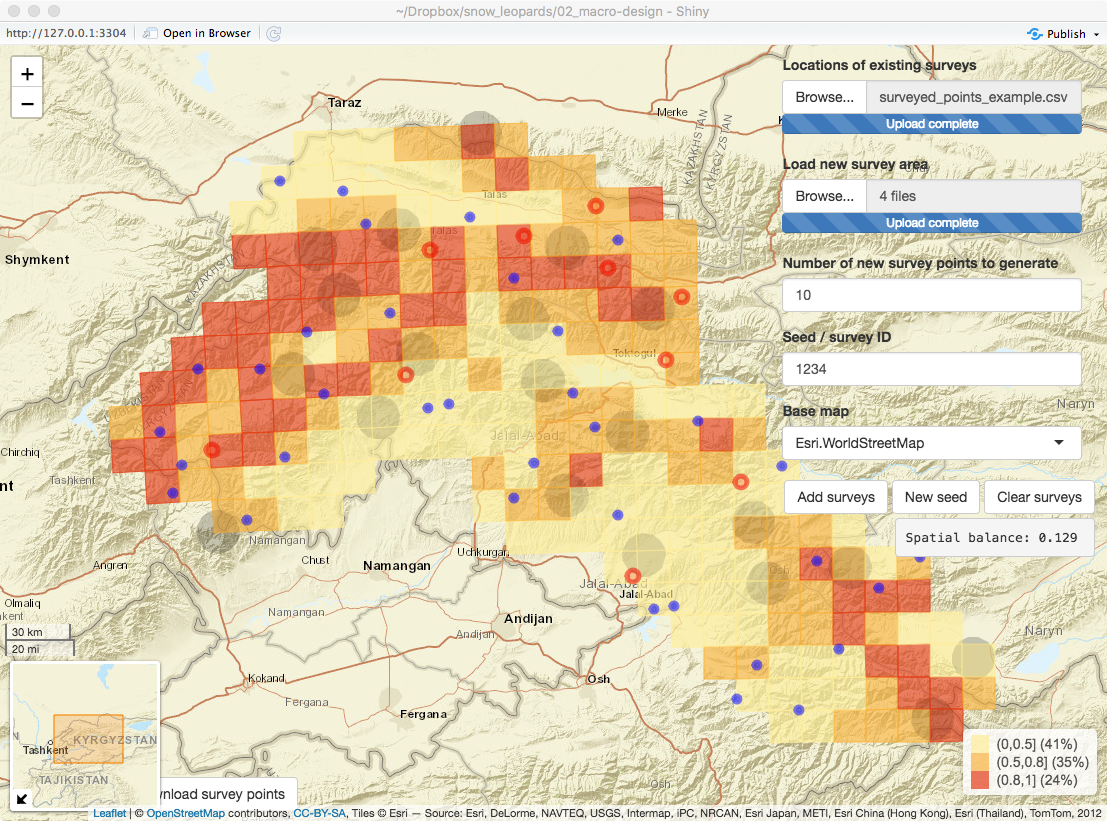
\includegraphics[width=\textwidth]{mac-9}
    \caption{Adding a further 10 survey points}
  \end{subfigure}
  \caption{Any areas already surveyed can be uploaded and excluded from the study area (a, denoted by grey polygons). Any desired number of new survey site locations can be generated by clicking the ``Add surveys'' button. New survey sites are always indicated in red. In (b) 25 new survey sites are selected. These denote the approximate centre of any camera trap survey area, with the exact locations of camera traps to be determined by some micro-level survey design. Additional survey site locations can be added while preserving the overall spatial balance of the sample sequentially, so that it is not necessary to know the exact number of surveys that will be done in advance. In (c) ten new survey points are added to the 25 existing points, which turn blue (existing survey locations are always coloured blue). In (d) a further ten points are added, to the now 35 existing survey points.}
\label{mac-6789}
\end{figure}
 
%\begin{figure}[htbp]
%\centering
%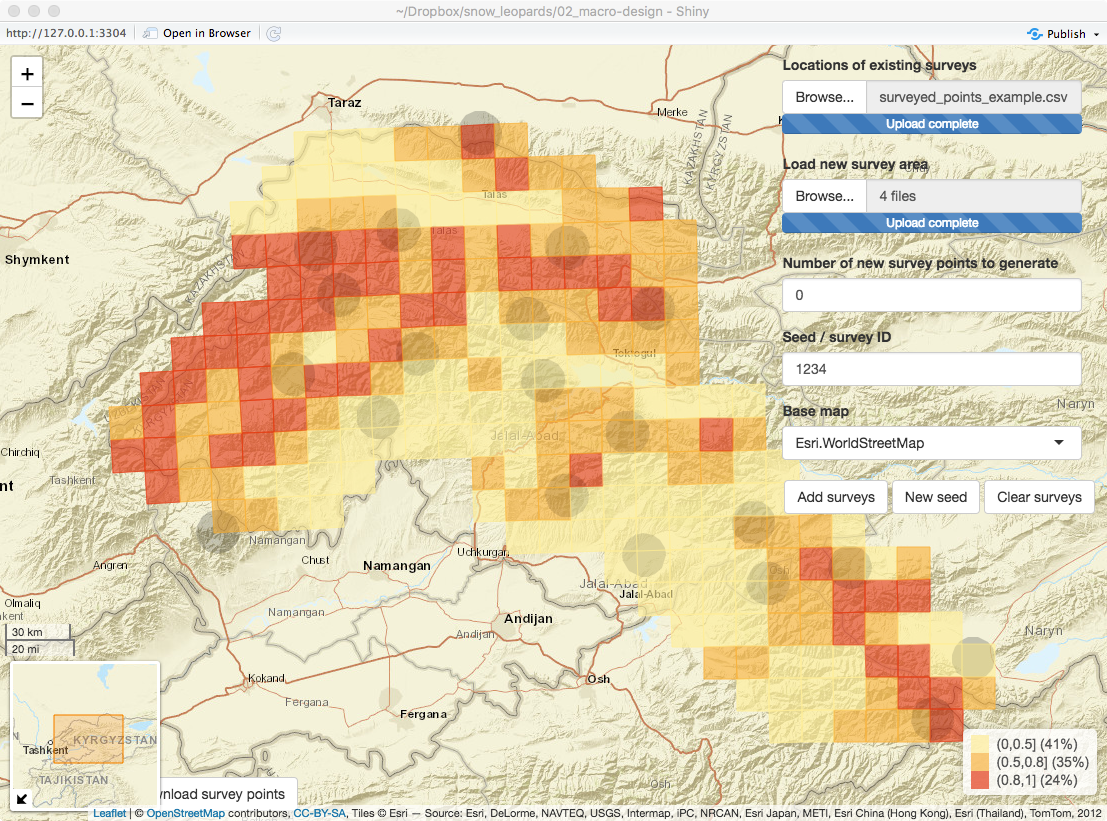
\includegraphics[width=\textwidth]{mac-6}
%\caption{}
%\label{mac-6}
%\end{figure}

\subsubsection{Generating sample sites}
A first set of survey sites can be generated as follows:
\begin{enumerate}
\item Click \textit{New seed}, which sets the randomization part of the design. This generates a survey ID, located in the \textit{Seed/survey ID} box. {\bf It is critical to record this number, which provides the only way of reproducing the survey points.}
\item Set the \textit{Number of new survey points to generate} box to the desired number.
\item Click \textit{Add surveys}. 
\end{enumerate}
New survey points appear as red circles (Figure \ref{mac-6789}b).

%\begin{figure}[htbp]
%\centering
%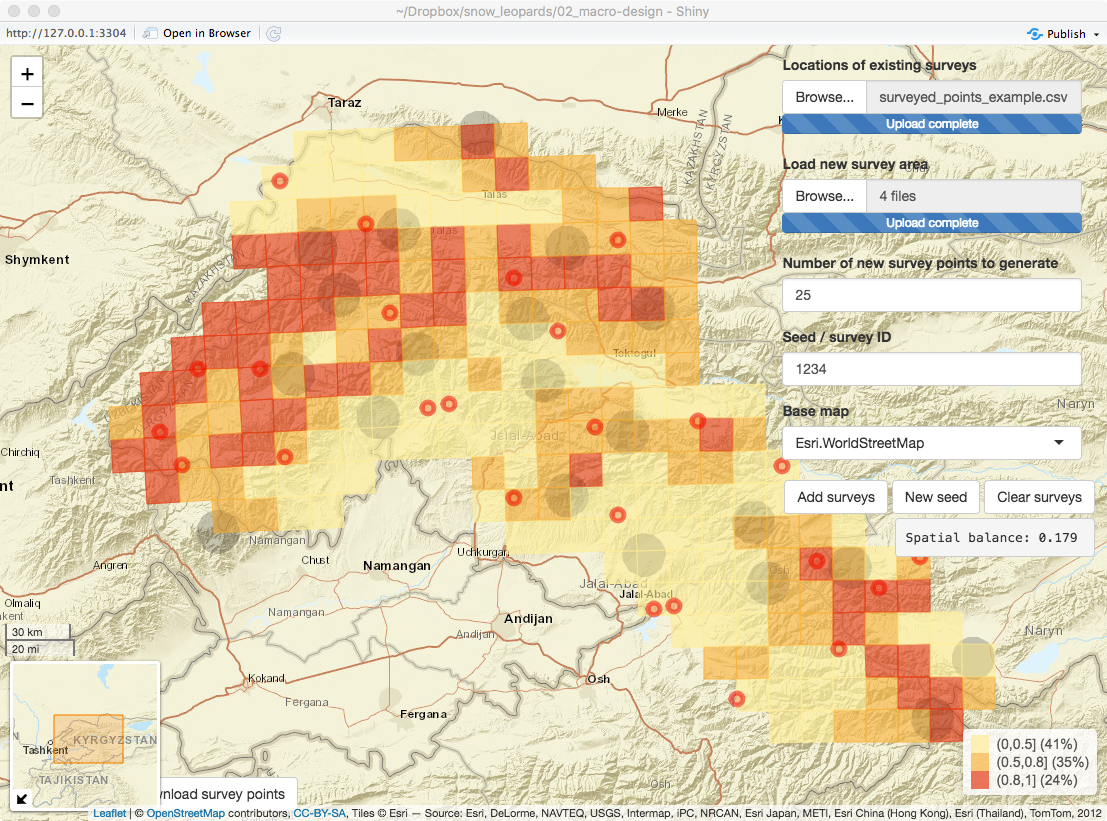
\includegraphics[width=\textwidth]{mac-7}
%\caption{}
%\label{mac-7}
%\end{figure} 

If all existing survey points are already visible on the map, then additional survey points can be generated by the following steps:
\begin{enumerate}
\item Set the \textit{Number of new survey points to generate} box to the desired number.
\item Click \textit{Add surveys}. 
\end{enumerate}
Existing survey points turn blue, and the survey points just added appear in red  (Figure \ref{mac-6789}c and d).
%\begin{figure}[htbp]
%\centering
%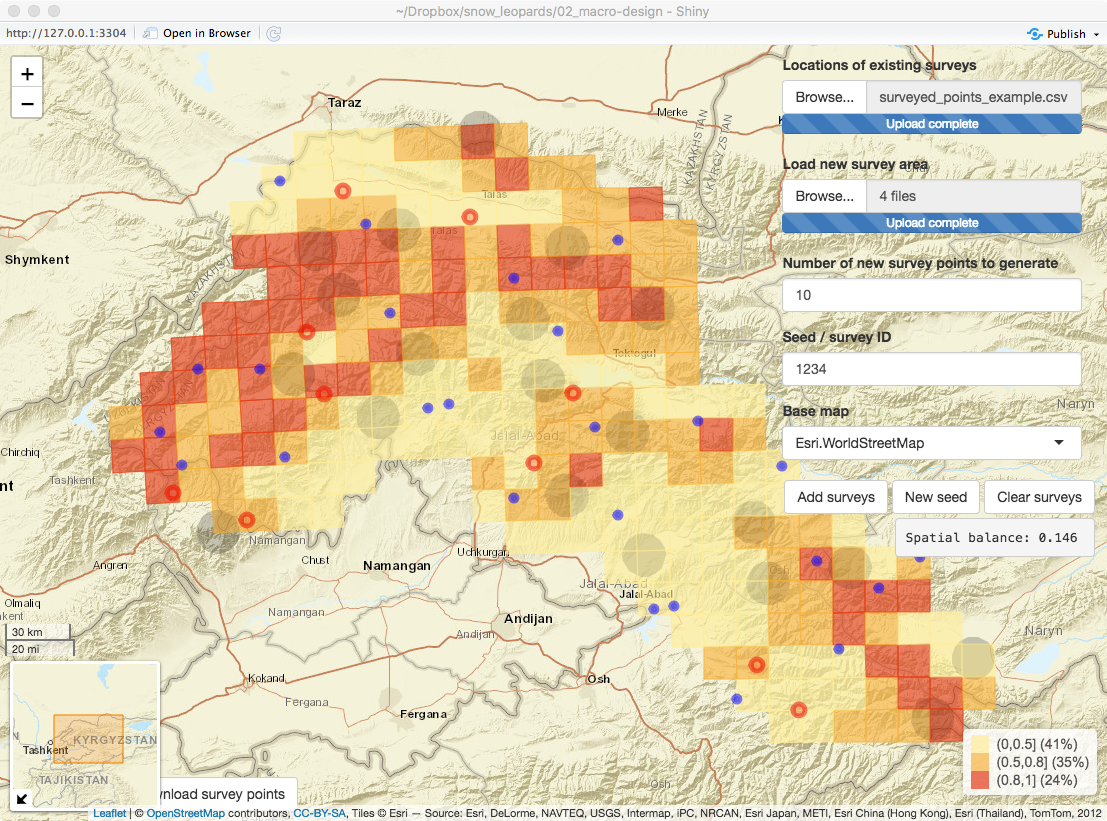
\includegraphics[width=\textwidth]{mac-8}
%\caption{}
%\label{mac-8}
%\end{figure} 

If existing survey points are not already visible on the map, for example if the user is using the app from time to time to generate supplementary survey points, then the previously generated points must first be re-generated before additional points can be added:
\begin{enumerate}
\item Recreate the existing survey points by entering the ID of the survey (recorded when first generating the original survey points) in the \textit{Seed/survey ID} box, and enter the number of surveys already done in the \textit{Number of new survey points to generate}. Selecting \textit{Add surveys} will add the locations of the existing surveys as red circles. Confirm that these are the correct locations.
\item Set the \textit{Number of new survey points to generate} box to the desired number.
\item Click \textit{Add surveys}. 
\end{enumerate}
Again, existing survey points turn blue and new survey points in red.

The app is designed to be used over time; for example a user might use the app at the beginning of a field season to generate a new set of points to survey. Because additional survey points are generated so that the entire sample is well-balanced, their locations depend on any exisiting survey points generated previously. For this reason, it is critical to make a note of the randomization seed that has been used to generate survey points to date. This is the number located in the \textit{Seed/survey ID} box. Coordinates of survey points can be exported in a csv file at any stage by clicking the \textit{Download survey points} button.


\bibliographystyle{abbrvnat}
\bibliography{secr_refs}  

\end{document}
\end{document}